%!TEX root = ../thesis.tex

\section{実験概要}
%\begin{figure}[hbtp]
  %\centering
 %\includegraphics[keepaspectratio, scale=0.8]
      %{images/RaspberryPiMouse.png}
 %\caption{Example}
 %\label{Fig:Example}
%\end{figure}
%\subsection{実験概要}

本章では,Navigation2 における各種パラメータ設定が,自律移動ロボットの走行挙動に与える影響を調査するために実施した走行実験について述べる.

以下では,まず実験の目的を示し,次に実験装置および実験環境について説明する.その後,実験方法とパラメータ設定条件を示すことで,本研究における実験の全体像を明らかにする.
%本研究では,本研究室で開発されているロボット ORNE-box3\cite{井口颯人2023屋外自律移動ロボットプラットフォーム-orne} を用いて走行実験を行った.実機ロボットの外観を\figref{Fig:ORNE-box3}に示す.
%ORNE-box3のセンサ構成については、\figref{Fig:sensor configuration}に示すように,PCとしてJetson Orin NX 16GBを搭載しており、3D LiDAR:R-Fans-16
%、IMU:ADIS16465、Encoder : i-Cart middleを備えている.3D LiDARは、自己位置推定と障害物検知に使用し、IMUとエンコーダは、emcl2に対して情報を提供している.
\subsection{実験目的}

本実験の目的は,ROS 2 Navigation2 における各種パラメータを個別に変化させた際に,自律移動中のロボットの挙動がどのように変化するかを明らかにすることである.

特に,走行速度,軌道の安定性,旋回挙動,およびゴール到達可否といった観点から,パラメータ設定がロボットの走行性能に与える影響を評価することを目的とする.
%走行ルートは\figref{Fig:Course map of the Tsudanuma Challenge 2025}が示すように,津田沼校舎2号館前から食堂前に設置されたコーンまでとし,
%津田沼チャレンジのコースの一部を利用した.このルートは,屋外環境における
%自律移動性能を評価するための実環境を想定したものである.


%実験では,Navigation2 における各種パラメータを個別に変化させた場合の
%ロボットの挙動の変化を調査することを目的とした.
%各走行実験においては,対象とするパラメータのみを変更し,
%それ以外のパラメータはすべて一定に保った.

%また,パラメータの変更に際しては,変更前の設定値を基準値とし,
%基準値から増減させた場合のロボットの走行挙動を比較・分析した.
%これにより,各パラメータがロボットの走行安定性や挙動に与える影響を
%明確にすることを試みた.

\subsection{実験装置}

\begin{figure}[H]
  \centering
 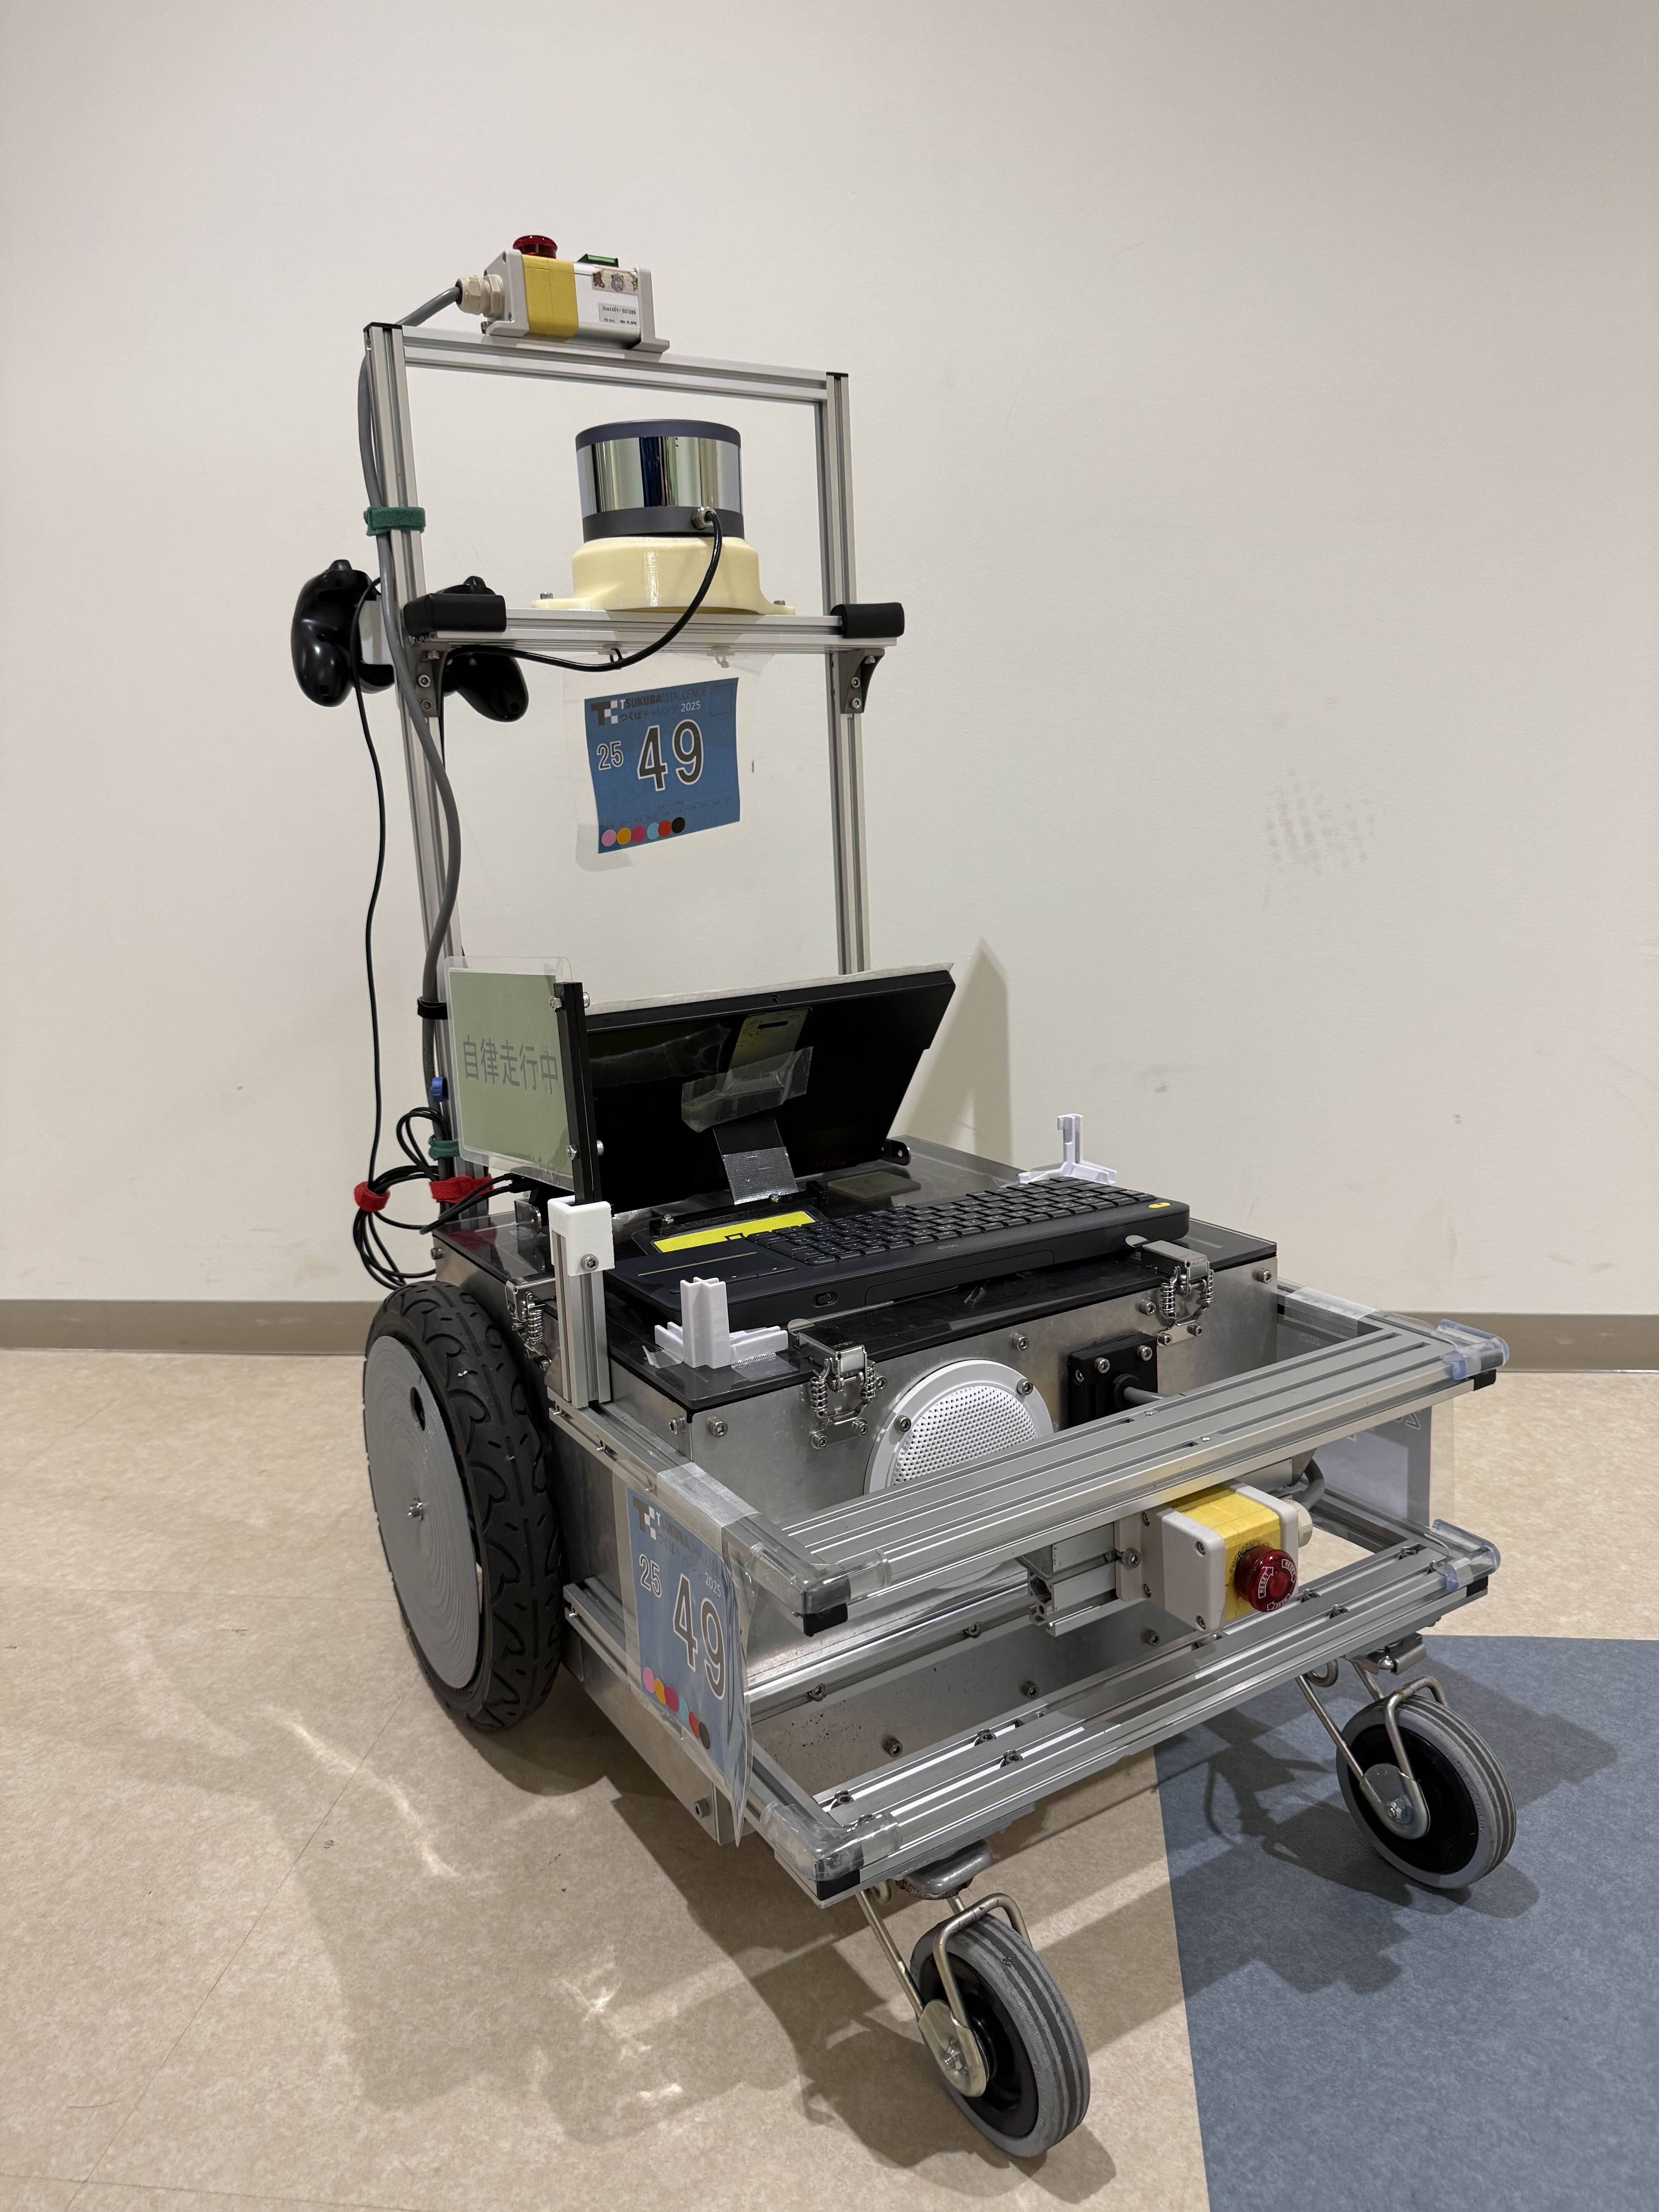
\includegraphics[keepaspectratio, scale=0.3]
      {images/orne-box3.png}
 \caption{ORNE-box3(source: \cite{井口颯人2023屋外自律移動ロボットプラットフォーム-orne})}
 \label{Fig:ORNE-box3}
\end{figure}
\begin{figure}[H]
  \centering
 \includegraphics[keepaspectratio, scale=0.3]
      {images/117.png}
 \caption{Overview of ORNE-box3 and its onboard sensors}
 \label{Fig:Overview of ORNE-box3 and its onboard sensors}
\end{figure}

実験には,本研究室で開発されている自律移動ロボット ORNE-box3\cite{井口颯人2023屋外自律移動ロボットプラットフォーム-orne} を使用した.ORNE-box3 の外観を\figref{Fig:ORNE-box3} に示す.

本ロボットは,計算機として Jetson Orin NX 16GB を搭載しており,自己位置推定およびナビゲーション処理を行う.また,周辺環境の認識および状態推定のために,3D LiDAR(R-Fans-16),IMU(ADIS16465),エンコーダ(i-Cart middle)を備えている.

3D LiDAR は自己位置推定および障害物検知に使用され,IMU とエンコーダから得られる情報は emcl2 に入力され,ロボットの自己位置推定に利用される.
\subsection{実験環境及び走行ルート}

\begin{figure}[H]
  \centering
 \includegraphics[keepaspectratio, scale=0.6]
      {images/tsudanumachallenge.png}
 \caption{Course map of the Tsudanuma Challenge 2025(source: \cite{Tsudanumachallenge})}
 \label{Fig:Course map of the Tsudanuma Challenge 2025}
\end{figure}

走行実験は\figref{Fig:Course map of the Tsudanuma Challenge 2025}に示すように,津田沼校舎 2 号館前から食堂前に設置されたコーンまでの区間で実施した.本ルートは,本研究室が参加している「津田沼チャレンジ」において使用されるコースの一部である.

津田沼チャレンジは,大学キャンパス内の実環境を対象として,自律移動ロボットの走行性能を検証する取り組みであり,歩行者や段差などが存在する屋外環境を想定している.本実験では,この実環境を模擬した走行ルートを用いることで,実運用に近い条件下での挙動評価を行った.


\subsection{実験方法}

実験では,Navigation2 における各種パラメータを個別に変化させた場合のロボットの走行挙動を観察した.

各走行実験においては,対象とするパラメータのみを変更し,それ以外のパラメータはすべて同一の設定とした.これにより,特定のパラメータ変更がロボットの挙動に与える影響を明確にすることを試みた.

また,各実験は同一の走行ルートおよび初期条件のもとで実施した.

パーティクル数は,パーティクルフィルタに基づく自己位置推定において,
仮説の多様性を決定する重要なパラメータである.
粒子数が不足した場合,自己位置推定が定性的に破綻し,ロボットが
ナビゲーションを継続できなくなる.
そのため,num\_particles に関する実験では,軌道の比較ではなく,
ゴール到達の可否を評価指標として用いた.こちらの実験回数は10回である.

その他のパラメータについては,自己位置推定が成立した状態での挙動
の違いを評価することを目的とし,rosbag に記録されたロボットの位置および向き
の時間変化を用いて解析を行った.こちらの実験回数は一回である.

\subsection{実験条件及びパラメータ設定}

%本研究において基準とした Navigation2 のパラメータ設定を表\ref{tab:base_parameters}に示す.

本研究において基準とした Navigation2 および emcl2 のパラメータを
Table\ref{tab:emcl2_parameters}〜Table\ref{tab:planner_goal_parameters}に示す。

また,実験番号と変更したパラメータの対応をTable\ref{tab:exp_emcl2}〜Table\ref{tab:exp_planner_goal}に示す.各実験では,表に示したパラメータのみを基準値から変更し,その他の設定はすべて基準値と同一とした.

\begin{table}[H]
  \centering
  \caption{Baseline Parameter Settings in emcl2}
  \label{tab:emcl2_parameters}
  \begin{tabular}{ll}
    \hline
    Parameter & Baseline Value \\
    \hline
    num\_particles & 500 \\
    odom\_fw\_dev\_per\_fw & 0.19 \\
    odom\_fw\_dev\_per\_rot & 0.0001 \\
    odom\_rot\_dev\_per\_fw & 0.13 \\
    odom\_rot\_dev\_per\_rot & 0.2 \\
    laser\_likelihood\_max\_dist & 0.2 \\
    range\_threshold & 0.3 \\
    \hline
  \end{tabular}
\end{table}

\begin{table}[H]
  \centering
  \caption{Baseline Parameter Settings for the Nav2 Controller}
  \label{tab:controller_parameters}
  \begin{tabular}{ll}
    \hline
    Parameter & Baseline Value \\
    \hline
    max\_vel\_x & 0.6 \\
    max\_vel\_theta & 0.7 \\
    max\_speed\_xy & 0.9 \\
    min\_theta\_velocity\_threshold & 0.001 \\
    acc\_lim\_x & 1.0 \\
    acc\_lim\_theta & 3.2 \\
    linear\_granularity & 0.05 \\
    angular\_granularity & 0.025 \\
    xy\_goal\_tolerance & 0.25 \\
    \hline
  \end{tabular}
\end{table}

\begin{table}[H]
  \centering
  \caption{Baseline Parameter Settings for the Nav2 Costmap}
  \label{tab:costmap_parameters}
  \begin{tabular}{lll}
    \hline
    Target & Parameter & Baseline Value \\
    \hline
    Global & global\_resolution & 0.1 \\
    Global & global\_cost\_scaling\_factor & 3.0 \\
    Global & global\_inflation\_radius & 0.5 \\
    Local & local\_resolution & 0.1 \\
    Local & local\_cost\_scaling\_factor & 3.0 \\
    Local & local\_inflation\_radius & 0.3 \\
    \hline
  \end{tabular}
\end{table}

\begin{table}[H]
  \centering
  \caption{Baseline Parameter Settings for the Nav2 Velocity Smoother}
  \label{tab:velocity_smoother_parameters}
  \begin{tabular}{ll}
    \hline
    Parameter & Baseline Value \\
    \hline
    smoothing\_frequency & 20 \\
    max\_velocity\_x & 0.6 \\
    max\_velocity\_theta & 1.7 \\
    max\_accel\_x & 0.5 \\
    max\_accel\_theta & 1.0 \\
    \hline
  \end{tabular}
\end{table}

\begin{table}[H]
  \centering
  \caption{Baseline Parameter Settings for the Nav2 Planner and Goal Evaluation}
  \label{tab:planner_goal_parameters}
  \begin{tabular}{ll}
    \hline
    Parameter & Baseline Value \\
    \hline
    trans\_stopped\_velocity & 0.25 \\
    planner\_tolerance & 0.5 \\
    \hline
  \end{tabular}
\end{table}

\begin{table}[H]
  \centering
  \caption{Experiments on emcl2 parameters}
  \label{tab:exp_emcl2}
  \begin{tabular}{lll}
    \hline
    Experiment ID & Parameter & Tested Values \\
    \hline
    E1 & Number of particles & 200, 1000 \\
    E2 & odom\_fw\_dev\_per\_fw & 0.01, 0.05, 0.1, 0.3, 0.4, 0.5 \\
    E3 & odom\_fw\_dev\_per\_rot & 0.001, 0.01, 0.1, 0.5 \\
    E4 & odom\_rot\_dev\_per\_fw & 0.01, 0.2, 0.3, 0.4, 0.5 \\
    E5 & odom\_rot\_dev\_per\_rot & 0.1, 0.3, 0.4, 0.5 \\
    E6 & laser\_likelihood\_max\_dist & 0.5, 1.0 \\
    E7 & range\_threshold & 0.5, 0.9 \\
    \hline
  \end{tabular}
\end{table}

\begin{table}[H]
  \centering
  \caption{Experiments on Nav2 controller parameters}
  \label{tab:exp_controller}
  \begin{tabular}{lll}
    \hline
    Experiment ID & Parameter & Tested Values \\
    \hline
    E8  & max\_vel\_x & 0.2, 1.0 \\
    E9  & max\_vel\_theta & 0.4, 1.0 \\
    E10 & max\_speed\_xy & 0.1, 0.5, 1.5 \\
    E11 & min\_theta\_velocity\_threshold & 0.01, 0.1, 1.0 \\
    E12 & acc\_lim\_x & 0.1, 0.5, 1.5 \\
    E13 & acc\_lim\_theta & 0.1, 1.0, 4.0 \\
    E14 & linear\_granularity & 0.01, 0.1, 0.5 \\
    E15 & angular\_granularity & 0.001, 0.01, 0.04 \\
    E16 & xy\_goal\_tolerance & 0.01, 0.1, 0.4 \\
    \hline
  \end{tabular}
\end{table}

\begin{table}[H]
  \centering
  \caption{Experiments on Nav2 costmap parameters}
  \label{tab:exp_costmap}
  \begin{tabular}{llll}
    \hline
    Experiment ID & Scope & Parameter & Tested Values \\
    \hline
    E17 & Global & global\_resolution & 0.05, 0.5, 1.0 \\
    E18 & Global & global\_cost\_scaling\_factor & 1.0, 5.0, 10.0 \\
    E19 & Global & global\_inflation\_radius & 0.1, 1.0, 2.0 \\
    E20 & Local  & local\_resolution & 0.05, 0.5, 1.0 \\
    E21 & Local  & local\_cost\_scaling\_factor & 1.0, 5.0, 10.0 \\
    E22 & Local  & local\_inflation\_radius & 0.1, 0.5, 1.0, 2.0 \\
    \hline
  \end{tabular}
\end{table}

\begin{table}[H]
  \centering
  \caption{Experiments on Nav2 velocity smoother parameters}
  \label{tab:exp_velocity_smoother}
  \begin{tabular}{lll}
    \hline
    Experiment ID & Parameter & Tested Values \\
    \hline
    E23 & smoothing\_frequency & 5, 10, 40, 60 \\
    E24 & max\_velocity\_x & 0.3, 0.9, 1.2 \\
    E25 & max\_velocity\_theta & 0.6, 2.5 \\
    E26 & max\_accel\_x & 0.2, 1.0 \\
    E27 & max\_accel\_theta & 0.5, 2.0 \\
    \hline
  \end{tabular}
\end{table}

\begin{table}[H]
  \centering
  \caption{Experiments on Nav2 planner and goal checker parameters}
  \label{tab:exp_planner_goal}
  \begin{tabular}{lll}
    \hline
    Experiment ID & Parameter & Tested Values \\
    \hline
    E28 & trans\_stopped\_velocity & 0.01, 0.1, 0.4 \\
    E29 & planner\_tolerance & 0.1, 1.0 \\
    \hline
  \end{tabular}
\end{table}



%\begin{figure}[hbtp]
  %\centering
 %\includegraphics[keepaspectratio, scale=0.6]
      %{images/tsudanumachallenge.png}
 %\caption{Course map of the Tsudanuma Challenge 2025(source: \cite{Tsudanumachallenge})}
 %\label{Fig:Course map of the Tsudanuma Challenge 2025}
%\end{figure}

%\begin{figure}[hbtp]
  %\centering
 %\includegraphics[keepaspectratio, scale=0.3]
      %{images/orne-box3.png}
 %\caption{ORNE-box3(source: \cite{井口颯人2023屋外自律移動ロボットプラットフォーム-orne})}
 %\label{Fig:ORNE-box3}
%\end{figure}
%\begin{figure}[hbtp]
  %\centering
 %\includegraphics[keepaspectratio, scale=0.3]
      %{images/sensor.png}
 %\caption{sensor configuration}
 %\label{Fig:sensor configuration}
%\end{figure}
%\subsubsection{etc...}


\newpage

\section{実験結果}
%\begin{figure}[hbtp]
  %\centering
 %\includegraphics[keepaspectratio, scale=0.8]
      %{images/RaspberryPiMouse.png}
 %\caption{Example}
 %\label{Fig:Example}
%\end{figure}
\subsection{実験結果(emcl2)}
\subsubsection{実験結果(num\_particles)}
基準となるパーティクル数は500である.
\begin{table}[H]
  \centering
  %\caption{パーティクル数の違いによるゴール到達可否}
  \caption{Goal Achievement under Different Particle Counts}
  \label{tab:num_particles_result}
  \begin{tabular}{c|c|c|c}
    \hline
    & \multicolumn{3}{c}{Number of particles} \\
    \hline
    Number of times  & 200 & 500 (base) & 1000 \\
    \hline
    1  & $\times$ & ○ & ○ \\
    2  & ○ & ○ & $\times$ \\
    3  & $\times$ & $\times$ & $\times$ \\
    4  & ○ & ○ & ○ \\
    5  & ○ & ○ & $\times$ \\
    6  & $\times$ & $\times$ & $\times$ \\
    7  & ○ & ○ & ○ \\
    8  & ○ & ○ & ○ \\
    9  & ○ & ○ & ○ \\
    10 & ○ & ○ & ○ \\
    \hline
  \end{tabular}
\end{table}

Table\ref{tab:num_particles_result}に、パーティクル数の違いによるゴール到達の可否を示す.

\begin{table}[H]
  \centering
  %\caption{パーティクル数ごとのゴール到達成功率}
  \caption{Goal Achievement Rate for Different Numbers of Particles}
  \label{tab:num_particles_success_rate}
  \begin{tabular}{c|c}
    \hline
    Number of Particles & Success Rate [\%] \\
    \hline
    200  & 70 \\
    500 (base) & 80 \\
    1000 & 60 \\
    \hline
  \end{tabular}
\end{table}

Table\ref{tab:num_particles_success_rate}に,
パーティクル数を変化させた際のゴール到達成功率を示す.

Table\ref{tab:num_particles_result}, Table\ref{tab:num_particles_success_rate}が示すように、パーティクル数を 200,500,1000 と変化させて自己位置推定の安定性を評価した.
その結果,パーティクル数 500 の場合に最も高いゴール到達率が得られた.
一方で,200 および 1000 の場合は,到達率がやや低下する傾向が確認された.
パーティクル数が少ないと自己位置推定が破綻しやすく、成功率が低下した.また、パーティクル数が多すぎても計算量の増加によって、遅延が発生して安定性が低下した。
以上より,パーティクル数は多ければ良いわけではなく,
自己位置推定の精度と計算負荷のバランスを考慮した適切な設定が重要であることが分かる.
本実験環境においては,パーティクル数 500 が最も安定した性能を示した.

次からの実験では, ロボットの位置と向きを比較する. \figref{Fig:Base orientation}, \figref{Fig:Base position}のグラフが基準の値の時のロボットの挙動である。\figref{Fig:Base orientation}はロボットの向き、\figref{Fig:Base orientation version map}は、コース上での矢印の時のロボットの向き、\figref{Fig:Base position}はロボットの位置のグラフ, \figref{Fig:Base position version map}地図とロボットの位置を合わせたものである. このロボットの位置のグラフにおけるゴールは, x座標-275~-270, y座標-380~-370である.
\begin{figure}[H]
  \centering
 \includegraphics[keepaspectratio, scale=0.6]
      {images/1.png}
 \caption{Base orientation}
 \label{Fig:Base orientation}
\end{figure}

\begin{figure}[H]
  \centering
 \includegraphics[keepaspectratio, scale=0.6]
      {images/118.png}
 \caption{Base orientation version map}
 \label{Fig:Base orientation version map}
\end{figure}
\begin{figure}[H]
  \centering
 \includegraphics[keepaspectratio, scale=0.6]
      {images/2.1.png}
 \caption{Base position}
 \label{Fig:Base position}
\end{figure}

\begin{figure}[H]
  \centering
 \includegraphics[keepaspectratio, scale=0.6]
      {images/base111.png}
 \caption{Base position version map}
 \label{Fig:Base position version map}
\end{figure}

\subsubsection{実験結果(odom\_fw\_dev\_per\_fw)}
Table\ref{tab:emcl2_parameters}が示すように基準の値は、0.19.
ロボットの位置と向きは、\figref{Fig:Base orientation}, \figref{Fig:Base position version map}で示す
\begin{figure}[H]
  \centering
 \includegraphics[keepaspectratio, scale=0.6]
      {images/fwfw0.01muki3.png}
 \caption{Robot orientation with fw\_dev\_per\_fw = 0.01}
 \label{Fig:Robot orientation with fw_dev_per_fw = 0.01 }
\end{figure}
\begin{figure}[H]
  \centering
 \includegraphics[keepaspectratio, scale=0.6]
      {images/fwfw0.01iti2.png}
 \caption{Robot position with fw\_dev\_per\_fw = 0.01
}
 \label{Fig:Robot position with fw_dev_per_fw = 0.01}
\end{figure}

\begin{figure}[H]
  \centering
 \includegraphics[keepaspectratio, scale=0.6]
      {images/fwfw0.05muki2.png}
 \caption{Robot orientation with fw\_dev\_per\_fw = 0.05}
 \label{Fig:Robot orientation with fw_dev_per_fw = 0.05 }
\end{figure}
\begin{figure}[H]
  \centering
 \includegraphics[keepaspectratio, scale=0.6]
      {images/fwfw0.05iti2.png}
 \caption{Robot position with fw\_dev\_per\_fw = 0.05
}
 \label{Fig:Robot position with fw_dev_per_fw = 0.05}
\end{figure}

\begin{figure}[H]
  \centering
 \includegraphics[keepaspectratio, scale=0.6]
      {images/fwfw0.1muki2.png}
 \caption{Robot orientation with fw\_dev\_per\_fw = 0.1}
 \label{Fig:Robot orientation with fw_dev_per_fw = 0.1 }
\end{figure}
\begin{figure}[H]
  \centering
 \includegraphics[keepaspectratio, scale=0.6]
      {images/fwfw0.1iti2.png}
 \caption{Robot position with fw\_dev\_per\_fw = 0.1
}
 \label{Fig:Robot position with fw_dev_per_fw = 0.1}
\end{figure}

\begin{figure}[H]
  \centering
 \includegraphics[keepaspectratio, scale=0.6]
      {images/fwfw0.3muki.png}
 \caption{Robot orientation with fw\_dev\_per\_fw = 0.3}
 \label{Fig:Robot orientation with fw_dev_per_fw = 0.3 }
\end{figure}
\begin{figure}[H]
  \centering
 \includegraphics[keepaspectratio, scale=0.6]
      {images/fwfw0.3iti.png}
 \caption{Robot position with fw\_dev\_per\_fw = 0.3
}
 \label{Fig:Robot position with fw_dev_per_fw = 0.3}
\end{figure}

\begin{figure}[H]
  \centering
 \includegraphics[keepaspectratio, scale=0.6]
      {images/fwfw0.4muki.png}
 \caption{Robot orientation with fw\_dev\_per\_fw = 0.4}
 \label{Fig:Robot orientation with fw_dev_per_fw = 0.4 }
\end{figure}
\begin{figure}[H]
  \centering
 \includegraphics[keepaspectratio, scale=0.6]
      {images/fwfw0.4iti.png}
 \caption{Robot position with fw\_dev\_per\_fw = 0.4
}
 \label{Fig:Robot position with fw_dev_per_fw = 0.4}
\end{figure}

\begin{figure}[H]
  \centering
 \includegraphics[keepaspectratio, scale=0.6]
      {images/fwfw0.5muki.png}
 \caption{Robot orientation with fw\_dev\_per\_fw = 0.5}
 \label{Fig:Robot orientation with fw_dev_per_fw = 0.5 }
\end{figure}
\begin{figure}[H]
  \centering
 \includegraphics[keepaspectratio, scale=0.6]
      {images/fwfw0.5iti.png}
 \caption{Robot position with fw\_dev\_per\_fw = 0.5
}
 \label{Fig:Robot position with fw_dev_per_fw = 0.5}
\end{figure}

\figref{Fig:Robot orientation with fw_dev_per_fw = 0.5 }で示すように、odom\_fw\_dev\_per\_fw を 0.5 に設定した場合,ロボットは走行を続けるにつれて自己位置推定の誤差が累積し,最終的にゴールに到達することができなかった.一方で,0.4 以下の値に設定した場合には,ロボットはゴールまで到達することが確認された.

また,直線走行時の挙動を基準条件と比較すると,odom\_fw\_dev\_per\_fw を大きく設定した場合には,推定されたロボットの位置が徐々にずれていく様子が確認された.このことから,odom\_fw\_dev\_per\_fw の値を過度に大きくすると,前進移動に対するオドメトリ誤差が強調され,自己位置推定の精度が低下することが示唆される.

%\figref{Fig:Robot orientation with fw_dev_per_fw = 0.01 },\figref{Fig:Robot position with fw_dev_per_fw = 0.01}

\subsubsection{実験結果(odom\_fw\_dev\_per\_rot)}
\figref{Fig:base orientation}, \figref{Fig:base position}で示すように、基準の値は、0.0001

\begin{figure}[H]
  \centering
 \includegraphics[keepaspectratio, scale=0.6]
      {images/fwrot0.001muki.png}
 \caption{Robot orientation with fw\_dev\_per\_rot = 0.001}
 \label{Fig:Robot orientation with fw_dev_per_rot = 0.001 }
\end{figure}
\begin{figure}[H]
  \centering
 \includegraphics[keepaspectratio, scale=0.6]
      {images/fwrot0.001iti.png}
 \caption{Robot position with fw\_dev\_per\_rot = 0.001
}
 \label{Fig:Robot position with fw_dev_per_rot = 0.001}
\end{figure}

\begin{figure}[H]
  \centering
 \includegraphics[keepaspectratio, scale=0.6]
      {images/fwrot0.01muki.png}
 \caption{Robot orientation with fw\_dev\_per\_rot = 0.01}
 \label{Fig:Robot orientation with fw_dev_per_rot = 0.01 }
\end{figure}
\begin{figure}[H]
  \centering
 \includegraphics[keepaspectratio, scale=0.6]
      {images/fwrot0.01iti.png}
 \caption{Robot position with fw\_dev\_per\_rot = 0.01
}
 \label{Fig:Robot position with fw_dev_per_rot = 0.01}
\end{figure}

\begin{figure}[H]
  \centering
 \includegraphics[keepaspectratio, scale=0.6]
      {images/fwrot0.1muki.png}
 \caption{Robot orientation with fw\_dev\_per\_rot = 0.1}
 \label{Fig:Robot orientation with fw_dev_per_rot = 0.1 }
\end{figure}
\begin{figure}[H]
  \centering
 \includegraphics[keepaspectratio, scale=0.6]
      {images/fwrot0.1iti.png}
 \caption{Robot position with fw\_dev\_per\_rot = 0.1
}
 \label{Fig:Robot position with fw_dev_per_rot = 0.1}
\end{figure}

\begin{figure}[H]
  \centering
 \includegraphics[keepaspectratio, scale=0.6]
      {images/fwrot0.5muki.png}
 \caption{Robot orientation with fw\_dev\_per\_rot = 0.5}
 \label{Fig:Robot orientation with fw_dev_per_rot = 0.5 }
\end{figure}
\begin{figure}[H]
  \centering
 \includegraphics[keepaspectratio, scale=0.6]
      {images/fwrot0.5iti.png}
 \caption{Robot position with fw\_dev\_per\_rot = 0.5
}
 \label{Fig:Robot position with fw_dev_per_rot = 0.5}
\end{figure}

odom\_fw\_dev\_per\_rot を変化させた実験では,すべての設定値においてロボットはゴールに到達することができた.特に,odom\_fw\_dev\_per\_rot を 0.5 に設定した場合には,走行中に自己位置推定のずれが一部確認されたものの,走行不能となるような大きな影響は見られず,最終的にゴールまで到達することが確認された.

この結果から,odom\_fw\_dev\_per\_rot は自己位置推定に一定の影響を与えるものの,fw 方向の移動誤差を表す odom\_fw\_dev\_per\_fw と比較すると,ゴール到達性に与える影響は相対的に小さいと考えられる.


\subsubsection{実験結果(odom\_rot\_dev\_per\_fw)}
\figref{Fig:base orientation}, \figref{Fig:base position}で示すように基準の値は、0.13

\begin{figure}[H]
  \centering
 \includegraphics[keepaspectratio, scale=0.6]
      {images/rotfw0.01muki.png}
 \caption{Robot orientation with rot\_dev\_per\_fw = 0.01}
 \label{Fig:Robot orientation with rot_dev_per_fw = 0.01 }
\end{figure}
\begin{figure}[H]
  \centering
 \includegraphics[keepaspectratio, scale=0.6]
      {images/rotfw0.01iti.png}
 \caption{Robot position with rot\_dev\_per\_fw = 0.01
}
 \label{Fig:Robot position with rot_dev_per_fw = 0.01}
\end{figure}

\begin{figure}[H]
  \centering
 \includegraphics[keepaspectratio, scale=0.6]
      {images/rotfw0.2muki.png}
 \caption{Robot orientation with rot\_dev\_per\_fw = 0.2}
 \label{Fig:Robot orientation with rot_dev_per_fw = 0.2 }
\end{figure}
\begin{figure}[H]
  \centering
 \includegraphics[keepaspectratio, scale=0.6]
      {images/rotfw0.2iti.png}
 \caption{Robot position with rot\_dev\_per\_fw = 0.2
}
 \label{Fig:Robot position with rot_dev_per_fw = 0.2}
\end{figure}

\begin{figure}[H]
  \centering
 \includegraphics[keepaspectratio, scale=0.6]
      {images/rotfw0.3muki.png}
 \caption{Robot orientation with rot\_dev\_per\_fw = 0.3}
 \label{Fig:Robot orientation with rot_dev_per_fw = 0.3 }
\end{figure}
\begin{figure}[H]
  \centering
 \includegraphics[keepaspectratio, scale=0.6]
      {images/rotfw0.3iti.png}
 \caption{Robot position with rot\_dev\_per\_fw = 0.3
}
 \label{Fig:Robot position with rot_dev_per_fw = 0.3}
\end{figure}

\begin{figure}[H]
  \centering
 \includegraphics[keepaspectratio, scale=0.6]
      {images/rotfw0.4muki.png}
 \caption{Robot orientation with rot\_dev\_per\_fw = 0.4}
 \label{Fig:Robot orientation with rot_dev_per_fw = 0.4 }
\end{figure}
\begin{figure}[H]
  \centering
 \includegraphics[keepaspectratio, scale=0.6]
      {images/rotfw0.4iti.png}
 \caption{Robot position with rot\_dev\_per\_fw = 0.4
}
 \label{Fig:Robot position with rot_dev_per_fw = 0.4}
\end{figure}

\begin{figure}[H]
  \centering
 \includegraphics[keepaspectratio, scale=0.6]
      {images/rotfw0.5muki.png}
 \caption{Robot orientation with rot\_dev\_per\_fw = 0.5}
 \label{Fig:Robot orientation with rot_dev_per_fw = 0.5 }
\end{figure}
\begin{figure}[H]
  \centering
 \includegraphics[keepaspectratio, scale=0.6]
      {images/rotfw0.5iti.png}
 \caption{Robot position with rot\_dev\_per\_fw = 0.5
}
 \label{Fig:Robot position with rot_dev_per_fw = 0.5}
\end{figure}

rot\_dev\_per\_fwでの実験では、rot\_dev\_per\_fw の値を大きくした場合においても,ロボットは直進走行中に自己位置および姿勢のわずかなずれが生じるのみであり,走行不能となることはなく,最終的にゴールまで問題なく到達することが確認された.

直線走行区間(目標方位 270°)でのロボットの向きに着目すると,rot\_dev\_per\_fw を 0.01 に設定した\figref{Fig:Robot orientation with rot_dev_per_fw = 0.01 }の場合には,ロボットは目標方位をほぼ維持したまま高い精度で直進していることが確認できた.一方で,rot\_dev\_per\_fw を 0.4 以上に設定した\figref{Fig:Robot orientation with rot_dev_per_fw = 0.4 },\figref{Fig:Robot orientation with rot_dev_per_fw = 0.5 }で示した場合には,走行中のロボットの方位が 270° を下回る傾向が見られ,進行に伴って姿勢が徐々にずれていく様子が確認された.

しかしながら,この方位のずれはナビゲーション全体に致命的な影響を与えるほどではなく,ゴール到達性に大きな影響は見られなかった.


\subsubsection{実験結果(odom\_rot\_dev\_per\_rot)}
\figref{Fig:base orientation}, \figref{Fig:base position}で示すように基準の値は、0.2

\begin{figure}[H]
  \centering
 \includegraphics[keepaspectratio, scale=0.6]
      {images/rotrot0.1muki2.png}
 \caption{Robot orientation with rot\_dev\_per\_rot = 0.1}
 \label{Fig:Robot orientation with rot_dev_per_rot = 0.1 }
\end{figure}
\begin{figure}[H]
  \centering
 \includegraphics[keepaspectratio, scale=0.6]
      {images/rotrot0.1iti.png}
 \caption{Robot position with rot\_dev\_per\_rot = 0.1
}
 \label{Fig:Robot position with rot_dev_per_rot = 0.1}
\end{figure}

\begin{figure}[H]
  \centering
 \includegraphics[keepaspectratio, scale=0.6]
      {images/rotrot0.3muki.png}
 \caption{Robot orientation with rot\_dev\_per\_rot = 0.3}
 \label{Fig:Robot orientation with rot_dev_per_rot = 0.3 }
\end{figure}
\begin{figure}[H]
  \centering
 \includegraphics[keepaspectratio, scale=0.6]
      {images/rotrot0.3iti.png}
 \caption{Robot position with rot\_dev\_per\_rot = 0.3
}
 \label{Fig:Robot position with rot_dev_per_rot = 0.3}
\end{figure}

\begin{figure}[H]
  \centering
 \includegraphics[keepaspectratio, scale=0.6]
      {images/rotrot0.4muki.png}
 \caption{Robot orientation with rot\_dev\_per\_rot = 0.4}
 \label{Fig:Robot orientation with rot_dev_per_rot = 0.4 }
\end{figure}
\begin{figure}[H]
  \centering
 \includegraphics[keepaspectratio, scale=0.6]
      {images/rotrot0.4iti.png}
 \caption{Robot position with rot\_dev\_per\_rot = 0.4
}
 \label{Fig:Robot position with rot_dev_per_rot = 0.4}
\end{figure}

\begin{figure}[H]
  \centering
 \includegraphics[keepaspectratio, scale=0.6]
      {images/rotrot0.5muki.png}
 \caption{Robot orientation with rot\_dev\_per\_rot = 0.5}
 \label{Fig:Robot orientation with rot_dev_per_rot = 0.5 }
\end{figure}
\begin{figure}[H]
  \centering
 \includegraphics[keepaspectratio, scale=0.6]
      {images/rotrot0.5iti.png}
 \caption{Robot position with rot\_dev\_per\_rot = 0.5
}
 \label{Fig:Robot position with rot_dev_per_rot = 0.5}
\end{figure}

%\subsection{rot\_dev\_per\_rot に関する実験結果}
rot\_dev\_per\_rot は,emcl において回転量に比例して付加される回転誤差を表すパラメータであり,
値が大きいほどセンサ情報を重視し,値が小さいほどオドメトリ情報を重視する設定となる.

本実験の結果,rot\_dev\_per\_rot の値を大きく設定した場合,
自己位置推定においてセンサの影響が強くなり,
ロボットの姿勢推定が不安定となることで,走行中の挙動がふらつく傾向が確認された.

特に旋回動作時においてセンサ重視の設定とした場合,
ゴール付近で自己位置推定が不安定となり,
rot\_dev\_per\_rot を 0.5 および 0.4 に設定した条件では,
ロボットがゴール端付近で停止し,正常にゴールへ到達できない事例が確認された.

以上より,rot\_dev\_per\_rot を過度に大きく設定すると,
回転時の姿勢推定においてセンサノイズの影響を受けやすくなり,
ナビゲーション性能が低下する可能性があることが示唆される.


\subsubsection{実験結果(laser\_likelihood\_max\_dist)}

\figref{Fig:base orientation}, \figref{Fig:base position}で示すように基準の値は、0.2

\begin{figure}[H]
  \centering
 \includegraphics[keepaspectratio, scale=0.6]
      {images/llmd0.5muki.png}
 \caption{Robot orientation with laser\_likelihood\_max\_dist = 0.5}
 \label{Fig:Robot orientation with laser_likelihood_max_dist = 0.5 }
\end{figure}
\begin{figure}[H]
  \centering
 \includegraphics[keepaspectratio, scale=0.6]
      {images/llmd0.5iti.png}
 \caption{Robot position with laser\_likelihood\_max\_dist = 0.5
}
 \label{Fig:Robot position with laser_likelihood_max_dist = 0.5}
\end{figure}

\begin{figure}[H]
  \centering
 \includegraphics[keepaspectratio, scale=0.6]
      {images/llmd1.0muki.png}
 \caption{Robot orientation with laser\_likelihood\_max\_dist = 1.0}
 \label{Fig:Robot orientation with laser_likelihood_max_dist = 1.0 }
\end{figure}
\begin{figure}[H]
  \centering
 \includegraphics[keepaspectratio, scale=0.6]
      {images/llmd1.0iti.png}
 \caption{Robot position with laser\_likelihood\_max\_dist = 1.0
}
 \label{Fig:Robot position with laser_likelihood_max_dist = 1.0}
\end{figure}


本実験では,基準値から laser\_likelihood\_max\_dist の値を増加させた場合,
レーザによって評価される情報量が増加し,
特に障害物や構造物が多く存在する環境において,
自己位置推定の更新が頻繁に行われることが確認された.

その結果,レーザスキャンによる評価負荷が高い箇所では,
ロボットが一時的に停止する挙動が観測された.
これは,自己位置推定の更新に伴い,
ナビゲーションが安全側に制御されたためであると考えられる.

一方で,laser\_likelihood\_max\_dist を約 0.5 程度まで増加させた場合でも,
ロボットは全体として安定した走行が可能であり,
大きなナビゲーション性能の低下は確認されなかった.

\subsubsection{実験結果(range\_threshold)}

\figref{Fig:base orientation}, \figref{Fig:base position}で示すように基準の値は、0.3
\begin{figure}[H]
  \centering
 \includegraphics[keepaspectratio, scale=0.6]
      {images/rt0.5muki.png}
 \caption{Robot orientation with range\_threshold = 0.5}
 \label{Fig:Robot orientation with range_threshold = 0.5 }
\end{figure}
\begin{figure}[H]
  \centering
 \includegraphics[keepaspectratio, scale=0.6]
      {images/rt0.5iti.png}
 \caption{Robot position with range\_threshold = 0.5
}
 \label{Fig:Robot position with range_threshold = 0.5}
\end{figure}

\begin{figure}[H]
  \centering
 \includegraphics[keepaspectratio, scale=0.6]
      {images/rt0.9muki.png}
 \caption{Robot orientation with range\_threshold = 0.9}
 \label{Fig:Robot orientation with range_threshold = 0.9 }
\end{figure}
\begin{figure}[H]
  \centering
 \includegraphics[keepaspectratio, scale=0.6]
      {images/rt0.9iti.png}
 \caption{Robot position with range\_threshold = 0.9
}
 \label{Fig:Robot position with range_threshold = 0.9}
\end{figure}

%\subsection{range\_threshold に関する実験結果}

本実験では、基準値である range\_threshold = 0.3 の場合,
ロボットは主に比較的近距離のレーザスキャン情報を用いて
自己位置推定を行っており,
推定された位置および姿勢は安定していた.

一方,range\_threshold を 0.9 に設定した場合,
より遠方のレーザスキャン情報も自己位置推定に使用されるため,
基準値の場合と比較して,
推定されたロボットの位置に明らかなずれが生じることや,
姿勢が異なる方向を示す場合が確認された.
しかしながら,これらのずれが生じた場合でも,
ロボットは最終的にゴール地点へ到達することができた.

また,range\_threshold を 0.5 に設定した場合には,
自己位置推定および走行挙動は安定しており,
基準値と比較して大きな性能低下は確認されなかった.

以上の結果より,range\_threshold は過度に大きな値を設定すると
自己位置推定の精度低下を招く可能性がある一方で,
0.5 程度までであれば,
安定したナビゲーションを維持したまま設定値を引き上げることが
可能であると考えられる.

emcl2の各パラメータの結果より,emcl2 における各パラメータは,
オドメトリ情報とレーザセンサ情報の信頼度のバランスを調整する役割を持ち,
設定値によって自己位置推定の特性および
ロボットの走行挙動が大きく変化することが明らかとなった.
そのため,実環境におけるナビゲーションでは,
各パラメータの意味を理解した上で,
環境特性に応じた適切な調整が重要であるといえる.

\subsection{実験結果(Nav2\_Controller)}

\subsubsection{実験結果(max\_vel\_x)}
\figref{Fig:base orientation}, \figref{Fig:base position}で示すように基準の値は、0.6

\begin{figure}[H]
  \centering
 \includegraphics[keepaspectratio, scale=0.6]
      {images/mvx0.2muki.png}
 \caption{Robot orientation with max\_vel\_x = 0.2}
 \label{Fig:Robot orientation with max_vel_x = 0.2 }
\end{figure}
\begin{figure}[H]
  \centering
 \includegraphics[keepaspectratio, scale=0.6]
      {images/mvx0.2iti.png}
 \caption{Robot position with max\_vel\_x = 0.2
}
 \label{Fig:Robot position with max_vel_x = 0.2}
\end{figure}


\begin{figure}[H]
  \centering
 \includegraphics[keepaspectratio, scale=0.6]
      {images/mvx1.0muki.png}
 \caption{Robot orientation with max\_vel\_x = 1.0}
 \label{Fig:Robot orientation with max_vel_x = 1.0 }
\end{figure}
\begin{figure}[H]
  \centering
 \includegraphics[keepaspectratio, scale=0.6]
      {images/mvx1.0iti.png}
 \caption{Robot position with max\_vel\_x = 1.0
}
 \label{Fig:Robot position with max_vel_x = 1.0}
\end{figure}

%\subsection{Controller における max\_vel\_x の実験結果}

%本実験では,Navigation2 の Controller における
%最大並進速度を制御するパラメータ max\_vel\_x を変更し,
%ロボットの走行挙動への影響を調査した.

まず,max\_vel\_x の値を小さく設定した場合,
ロボットの走行速度が低下し,
走行中の挙動が不安定になる傾向が確認された.
しかしながら,速度が低下した状態であっても,
ロボットはゴールまで到達することができ,
ナビゲーション自体が破綻することはなかった.

一方で,max\_vel\_x の値を基準値より大きく設定した場合,
走行挙動に大きな変化は見られず,
ロボットの実際の走行速度も基準値である 0.6\,[m/s] 以上には上昇しなかった.
この結果から,
max\_vel\_x を増加させても,
他のパラメータやシステム制約によって
ロボットの最大速度が制限されている可能性が考えられる.

以上のことから,
max\_vel\_x は走行速度の上限を設定する重要なパラメータである一方で,
ロボットの実際の最高速度は,
Controller 以外のパラメータや
ハードウェア設定の影響も受けることが示唆された.
この速度制限の要因については,
後述する実験において詳細に検証する.


\subsubsection{実験結果(max\_vel\_theta)}
\figref{Fig:base orientation}, \figref{Fig:base position}で示すように基準の値は、0.7

\begin{figure}[H]
  \centering
 \includegraphics[keepaspectratio, scale=0.6]
      {images/mvt0.4muki.png}
 \caption{Robot orientation with max\_vel\_theta = 0.4}
 \label{Fig:Robot orientation with max_vel_theta = 0.4 }
\end{figure}
\begin{figure}[H]
  \centering
 \includegraphics[keepaspectratio, scale=0.6]
      {images/mvt0.4iti.png}
 \caption{Robot position with max\_vel\_theta = 0.4
}
 \label{Fig:Robot position with max_vel_theta = 0.4}
\end{figure}

\begin{figure}[H]
  \centering
 \includegraphics[keepaspectratio, scale=0.6]
      {images/mvt1.0muki.png}
 \caption{Robot orientation with max\_vel\_theta = 1.0}
 \label{Fig:Robot orientation with max_vel_theta = 1.0 }
\end{figure}
\begin{figure}[H]
  \centering
 \includegraphics[keepaspectratio, scale=0.6]
      {images/mvt1.0iti.png}
 \caption{Robot position with max\_vel\_theta = 1.0
}
 \label{Fig:Robot position with max_vel_theta = 1.0}
\end{figure}

%\subsection{Controller における max\_vel\_theta の実験結果}
%本実験では,Navigation2 の Controller における
%最大角速度を制御するパラメータ max\_vel\_theta を変更し,
%ロボットの旋回挙動への影響を調査した.

本実験で、max\_vel\_theta の値を基準値より大きく設定した場合,
ロボットの走行挙動に顕著な変化は見られなかった.
この結果から,
基準値の時点でロボットの旋回性能は十分に確保されており,
それ以上角速度の上限を引き上げても,
実際の挙動には大きく反映されないことが示唆される.

一方で,max\_vel\_theta の値を基準値より小さく設定した場合,
ロボットの挙動が不安定になる様子が確認された.
特に,旋回が必要となる箇所において,
ロボットが一時的に停止し,
旋回完了までに時間を要する場面が多く見られた.
さらに,旋回後の直進動作においても,
進行方向が安定せず,
ふらついた挙動を示す傾向が確認された.

以上の結果より,
max\_vel\_theta を過度に小さく設定すると,
旋回動作およびその後の直進動作に悪影響を及ぼし,
ナビゲーション全体の安定性が低下することが明らかとなった.
そのため,本パラメータは,
旋回性能を確保できる十分な値に設定することが重要である.


\subsubsection{実験結果(max\_speed\_xy)}
\figref{Fig:base orientation}, \figref{Fig:base position}で示すように基準の値は、0.9

%0.1,0.5,1.5

\begin{figure}[H]
  \centering
 \includegraphics[keepaspectratio, scale=0.6]
      {images/msxy0.1muki.png}
 \caption{Robot orientation with max\_speed\_xy = 0.1}
 \label{Fig:Robot orientation with max_speed_xy = 0.1 }
\end{figure}
\begin{figure}[H]
  \centering
 \includegraphics[keepaspectratio, scale=0.6]
      {images/msxy0.1iti.png}
 \caption{Robot position with max\_speed\_xy = 0.1
}
 \label{Fig:Robot position with max_speed_xy = 0.1}
\end{figure}

\begin{figure}[H]
  \centering
 \includegraphics[keepaspectratio, scale=0.6]
      {images/msxy0.5muki.png}
 \caption{Robot orientation with max\_speed\_xy = 0.5}
 \label{Fig:Robot orientation with max_speed_xy = 0.5 }
\end{figure}
\begin{figure}[H]
  \centering
 \includegraphics[keepaspectratio, scale=0.6]
      {images/msxy0.5iti.png}
 \caption{Robot position with max\_speed\_xy = 0.5
}
 \label{Fig:Robot position with max_speed_xy = 0.5}
\end{figure}

\begin{figure}[H]
  \centering
 \includegraphics[keepaspectratio, scale=0.6]
      {images/msxy1.5muki.png}
 \caption{Robot orientation with max\_speed\_xy = 1.5}
 \label{Fig:Robot orientation with max_speed_xy = 1.5 }
\end{figure}
\begin{figure}[H]
  \centering
 \includegraphics[keepaspectratio, scale=0.6]
      {images/msxy1.5iti.png}
 \caption{Robot position with max\_speed\_xy = 1.5
}
 \label{Fig:Robot position with max_speed_xy = 1.5}
\end{figure}

%\subsection{Controller における max\_speed\_xy の実験結果}

%本実験では,Navigation2 の Controller において,
%並進方向の合成速度の上限を制御するパラメータ max\_speed\_xy を変更し,
%ロボットの走行挙動への影響を調査した.

本実験では、max\_speed\_xy を 0.5 に設定した場合,
ロボットは安定した走行を維持したままゴールへ到達することができた.
また,max\_speed\_xy を 1.5 に設定した場合においても,
ロボットの実際の走行速度に大きな変化は見られなかった.
この挙動は,
前節で述べた max\_vel\_x の実験結果と同様であり,
他のパラメータやシステム制約によって
ロボットの最大速度が制限されている可能性が考えられる.
この点については,後述する実験において検証を行う.

一方で,max\_speed\_xy を 0.1 に設定した場合,
ロボットの走行速度が極端に低下し,
ゴールまで到達することができなかった.
特に,走行開始後の初期段階において,
最初の曲がり角付近の段差に接触する挙動が確認された.
また,この設定値では,
曲がり角に進入する際に左右の車輪を交互に動かすような挙動が見られ,
滑らかな旋回動作が行われていなかった.

以上の結果より,
max\_speed\_xy を過度に小さく設定すると,
旋回動作が不安定となり,
ナビゲーションの遂行が困難になることが明らかとなった.
一方で,本パラメータを大きく設定した場合でも,
他の速度制限要因によって
実際の走行速度が制約される可能性があるため,
他の速度関連パラメータとの関係を考慮した調整が重要である.



\subsubsection{実験結果(min\_theta\_velocity\_threshold)}
\figref{Fig:base orientation}, \figref{Fig:base position}で示すように基準の値は、0.001

%0.01,0.1,1.0,
\begin{figure}[H]
  \centering
 \includegraphics[keepaspectratio, scale=0.6]
      {images/mtvt0.01muki.png}
 \caption{Robot orientation with min\_theta\_velocity\_threshold = 0.01}
 \label{Fig:Robot orientation with min_theta_velocity_threshold = 0.01 }
\end{figure}
\begin{figure}[H]
  \centering
 \includegraphics[keepaspectratio, scale=0.6]
      {images/mtvt0.01iti.png}
 \caption{Robot position with min\_theta\_velocity\_threshold = 0.01
}
 \label{Fig:Robot position with min_theta_velocity_threshold = 0.01}
\end{figure}
\begin{figure}[H]
  \centering
 \includegraphics[keepaspectratio, scale=0.6]
      {images/mtvt0.1muki.png}
 \caption{Robot orientation with min\_theta\_velocity\_threshold = 0.1}
 \label{Fig:Robot orientation with min_theta_velocity_threshold = 0.1 }
\end{figure}
\begin{figure}[H]
  \centering
 \includegraphics[keepaspectratio, scale=0.6]
      {images/mtvt0.1iti.png}
 \caption{Robot position with min\_theta\_velocity\_threshold = 0.1
}
 \label{Fig:Robot position with min_theta_velocity_threshold = 0.1}
\end{figure}
\begin{figure}[H]
  \centering
 \includegraphics[keepaspectratio, scale=0.6]
      {images/mtvt1.0muki.png}
 \caption{Robot orientation with min\_theta\_velocity\_threshold = 1.0}
 \label{Fig:Robot orientation with min_theta_velocity_threshold = 1.0 }
\end{figure}
\begin{figure}[H]
  \centering
 \includegraphics[keepaspectratio, scale=0.6]
      {images/mtvt1.0iti.png}
 \caption{Robot position with min\_theta\_velocity\_threshold = 1.0
}
 \label{Fig:Robot position with min_theta_velocity_threshold = 1.0}
\end{figure}
%\subsection{Controller における min\_theta\_velocity\_threshold の実験結果}

%本実験では,Navigation2 の Controller において,
%角速度の最小閾値を定義するパラメータ
%min\_theta\_velocity\_threshold を変更し,
%ロボットの旋回挙動への影響を調査した.

本実験では、基準値である min\_theta\_velocity\_threshold = 0.001 に対し,
本実験では 0.01,0.1,1.0 の各値について走行実験を行った.
その結果,基準値から値を段階的に増加させた場合においても,
ロボットの走行挙動に大きな変化は確認されなかった.

特に,min\_theta\_velocity\_threshold を 1.0 に設定した場合,
旋回動作時にロボットが停止する挙動が生じることが予想されたが,
実際には旋回および直進動作ともに問題なく行われ,
ロボットはゴール地点まで到達することができた.

以上の結果より,
min\_theta\_velocity\_threshold は,
今回の実験環境および走行条件においては,
一定範囲内で値を変化させても
ロボットの挙動に与える影響が比較的小さいパラメータであることが示唆された.


\subsubsection{実験結果(acc\_lim\_x)}
\figref{Fig:base orientation}, \figref{Fig:base position}で示すように基準の値は、1.0

%0.1,0.5,1.5,

\begin{figure}[H]
  \centering
 \includegraphics[keepaspectratio, scale=0.6]
      {images/alx0.1muki.png}
 \caption{Robot orientation with acc\_lim\_x = 0.1}
 \label{Fig:Robot orientation with acc_lim_x = 0.1 }
\end{figure}
\begin{figure}[H]
  \centering
 \includegraphics[keepaspectratio, scale=0.6]
      {images/alx0.1iti.png}
 \caption{Robot position with acc\_lim\_x = 0.1
}
 \label{Fig:Robot position with acc_lim_x = 0.1}
\end{figure}

\begin{figure}[H]
  \centering
 \includegraphics[keepaspectratio, scale=0.6]
      {images/alx0.5muki.png}
 \caption{Robot orientation with acc\_lim\_x = 0.5}
 \label{Fig:Robot orientation with acc_lim_x = 0.5 }
\end{figure}
\begin{figure}[H]
  \centering
 \includegraphics[keepaspectratio, scale=0.6]
      {images/alx0.5iti.png}
 \caption{Robot position with acc\_lim\_x = 0.5
}
 \label{Fig:Robot position with acc_lim_x = 0.5}
\end{figure}
\begin{figure}[H]
  \centering
 \includegraphics[keepaspectratio, scale=0.6]
      {images/alx1.5muki.png}
 \caption{Robot orientation with acc\_lim\_x = 1.5}
 \label{Fig:Robot orientation with acc_lim_x = 1.5 }
\end{figure}
\begin{figure}[H]
  \centering
 \includegraphics[keepaspectratio, scale=0.6]
      {images/alx1.5iti.png}
 \caption{Robot position with acc\_lim\_x = 1.5
}
 \label{Fig:Robot position with acc_lim_x = 1.5}
\end{figure}
%\subsection{Controller における acc\_lim\_x の実験結果}

%本実験では,Navigation2 の Controller において,
%並進方向の加速度制限を定義するパラメータ acc\_lim\_x を変更し,
%ロボットの走行挙動への影響を調査した.

本実験では、acc\_lim\_x の値を変化させた場合,
曲がり角通過後の直進動作において,
ロボットの加速がやや速く感じられる場面が確認された.
しかしながら,それ以外の走行挙動においては
顕著な変化は見られず,
いずれの設定値においても
ロボットは安定した走行を維持したまま
ゴール地点へ到達することができた.

以上の結果より,
acc\_lim\_x はロボットの加速特性を決定する上で
必要なパラメータであるものの,
本実験条件においては,
走行経路の追従性能や
ナビゲーション全体の安定性に与える影響は比較的小さいことが示唆された.



\subsubsection{実験結果(acc\_lim\_theta)}
\figref{Fig:base orientation}, \figref{Fig:base position}で示すように基準の値は、3.2

%0.1,1.0,4.0,
\begin{figure}[H]
  \centering
 \includegraphics[keepaspectratio, scale=0.6]
      {images/alt0.1muki.png}
 \caption{Robot orientation with acc\_lim\_theta = 0.1}
 \label{Fig:Robot orientation with acc_lim_theta = 0.1 }
\end{figure}
\begin{figure}[H]
  \centering
 \includegraphics[keepaspectratio, scale=0.6]
      {images/alt0.1iti.png}
 \caption{Robot position with acc\_lim\_theta = 0.1
}
 \label{Fig:Robot position with acc_lim_theta = 0.1}
\end{figure}
\begin{figure}[H]
  \centering
 \includegraphics[keepaspectratio, scale=0.6]
      {images/alt1.0muki.png}
 \caption{Robot orientation with acc\_lim\_theta = 1.0}
 \label{Fig:Robot orientation with acc_lim_theta = 1.0 }
\end{figure}
\begin{figure}[H]
  \centering
 \includegraphics[keepaspectratio, scale=0.6]
      {images/alt1.0iti.png}
 \caption{Robot position with acc\_lim\_theta = 1.0
}
 \label{Fig:Robot position with acc_lim_theta = 1.0}
\end{figure}
\begin{figure}[H]
  \centering
 \includegraphics[keepaspectratio, scale=0.6]
      {images/alt4.0muki.png}
 \caption{Robot orientation with acc\_lim\_theta = 4.0}
 \label{Fig:Robot orientation with acc_lim_theta = 4.0 }
\end{figure}
\begin{figure}[H]
  \centering
 \includegraphics[keepaspectratio, scale=0.6]
      {images/alt4.0iti.png}
 \caption{Robot position with acc\_lim\_theta = 4.0
}
 \label{Fig:Robot position with acc_lim_theta = 4.0}
\end{figure}
%\subsection{Controller における acc\_lim\_theta の実験結果}

%本実験では,Navigation2 の Controller において,
%角加速度の制限を定義するパラメータ acc\_lim\_theta を変更し,
%ロボットの旋回挙動への影響を調査した.

本実験では、acc\_lim\_theta を 0.1 に設定した場合,
最終的な旋回動作後の直進区間において,
ロボットの進行方向が細かく変化する,
いわゆるくねくねとした挙動が確認された.
その後,姿勢が安定し,
最終的にはゴール地点へ到達することができた.

また,acc\_lim\_theta を 1 に設定した場合においても,
走行中の進行方向が細かく変化する挙動が確認され,
これは取得したグラフからも明確に観察された.
しかしながら,この設定値においても,
ナビゲーション自体に支障はなく,
ロボットは問題なくゴールへ到達した.

一方で,acc\_lim\_theta を 4 に設定した場合,
走行挙動に大きな変化は見られず,
旋回および直進動作ともに安定した走行が確認された.

以上の結果より,
acc\_lim\_theta を過度に小さく設定すると,
旋回後の姿勢制御が不安定になりやすい一方で,
一定以上の値に設定することで,
安定した旋回挙動を維持できることが示唆された.

\subsubsection{実験結果(linear\_granularity)}
\figref{Fig:base orientation}, \figref{Fig:base position}で示すように基準の値は、0.05

%0.01,0.1,0.5,
\begin{figure}[H]
  \centering
 \includegraphics[keepaspectratio, scale=0.6]
      {images/lg0.01muki.png}
 \caption{Robot orientation with linear\_granularity = 0.01}
 \label{Fig:Robot orientation with linear_granularity = 0.01 }
\end{figure}
\begin{figure}[H]
  \centering
 \includegraphics[keepaspectratio, scale=0.6]
      {images/lg0.01iti.png}
 \caption{Robot position with linear\_granularity = 0.01
}
 \label{Fig:Robot position with linear_granularity = 0.01}
\end{figure}
\begin{figure}[H]
  \centering
 \includegraphics[keepaspectratio, scale=0.6]
      {images/lg0.1muki.png}
 \caption{Robot orientation with linear\_granularity = 0.1}
 \label{Fig:Robot orientation with linear_granularity = 0.1 }
\end{figure}
\begin{figure}[H]
  \centering
 \includegraphics[keepaspectratio, scale=0.6]
      {images/lg0.1iti.png}
 \caption{Robot position with linear\_granularity = 0.1
}
 \label{Fig:Robot position with linear_granularity = 0.1}
\end{figure}
\begin{figure}[H]
  \centering
 \includegraphics[keepaspectratio, scale=0.6]
      {images/lg0.5muki.png}
 \caption{Robot orientation with linear\_granularity = 0.5}
 \label{Fig:Robot orientation with linear_granularity = 0.5 }
\end{figure}
\begin{figure}[H]
  \centering
 \includegraphics[keepaspectratio, scale=0.6]
      {images/lg0.5iti.png}
 \caption{Robot position with linear\_granularity = 0.5
}
 \label{Fig:Robot position with linear_granularity = 0.5}
\end{figure}
%\subsection{Planner における linear\_granularity の実験結果}

%本実験では,Navigation2 の Planner において,
%経路生成時の並進方向の分解能を定義するパラメータ
%linear\_granularity を変更し,
%ロボットの走行挙動への影響を調査した.

%本実験では、基準値である linear\_granularity = 0.05 に対し,
%0.1 および 0.5 の各値について走行実験を行った.
本実験では、linear\_granularity を 0.5 に設定した場合,
走行開始後の最初の旋回箇所において
ロボットが一時的に停止する挙動が確認され,
その後,再び動き出すまでに時間を要した.
この挙動は,
経路の分解能が粗くなったことにより,
滑らかな経路生成が困難になったためであると考えられる.

一方で,linear\_granularity を 0.1 に設定した場合,
走行挙動は安定しており,
旋回動作を含めた経路においても
スムーズな走行が確認された.
この結果から,
linear\_granularity を基準値よりやや大きく設定した場合でも,
安定したナビゲーションが可能であることが示唆された.

以上の結果より,
linear\_granularity を過度に大きく設定すると,
経路生成の精度低下により
走行挙動が不安定になる可能性がある一方で,
0.1 程度の設定値であれば,
計算負荷と走行安定性の両立が可能であると考えられる.



\subsubsection{実験結果(angular\_granularity)}
\figref{Fig:base orientation}, \figref{Fig:base position}で示すように基準の値は、0.025

%0.001,0.01,0.04,
\begin{figure}[H]
  \centering
 \includegraphics[keepaspectratio, scale=0.6]
      {images/ag0.001muki.png}
 \caption{Robot orientation with angular\_granularity = 0.001}
 \label{Fig:Robot orientation with angular_granularity = 0.001 }
\end{figure}
\begin{figure}[H]
  \centering
 \includegraphics[keepaspectratio, scale=0.6]
      {images/ag0.001iti.png}
 \caption{Robot position with angular\_granularity = 0.001
}
 \label{Fig:Robot position with angular_granularity = 0.001}
\end{figure}

\begin{figure}[H]
  \centering
 \includegraphics[keepaspectratio, scale=0.6]
      {images/ag0.01muki.png}
 \caption{Robot orientation with angular\_granularity = 0.01}
 \label{Fig:Robot orientation with angular_granularity = 0.01 }
\end{figure}
\begin{figure}[H]
  \centering
 \includegraphics[keepaspectratio, scale=0.6]
      {images/ag0.01iti.png}
 \caption{Robot position with angular\_granularity = 0.01
}
 \label{Fig:Robot position with angular_granularity = 0.01}
\end{figure}

\begin{figure}[H]
  \centering
 \includegraphics[keepaspectratio, scale=0.6]
      {images/ag0.04muki.png}
 \caption{Robot orientation with angular\_granularity = 0.04}
 \label{Fig:Robot orientation with angular_granularity = 0.04 }
\end{figure}
\begin{figure}[H]
  \centering
 \includegraphics[keepaspectratio, scale=0.6]
      {images/ag0.04iti.png}
 \caption{Robot position with angular\_granularity = 0.04
}
 \label{Fig:Robot position with angular_granularity = 0.04}
\end{figure}

%\subsection{Planner における angular\_granularity の実験結果}

%本実験では,Navigation2 の Planner において,
%経路生成時の角度方向の分解能を定義するパラメータ
%angular\_granularity を変更し,
%ロボットの走行挙動への影響を調査した.

本実験では、angular\_granularity の値を基準値より小さく設定した場合,
ロボットの走行挙動に大きな変化は見られず,
旋回および直進動作ともに
安定した走行が確認された.
この結果から,
角度分解能を高めても,
本実験環境においては
挙動への影響は限定的であることが示唆される.

一方で,angular\_granularity を 4.0 に設定した場合,
最終的な旋回区間において,
ロボットの進行方向に
わずかな変化が生じていることが確認された.
この挙動は,
angular\_granularity = 4.0 の設定における
ロボットの姿勢変化を示したグラフからも確認でき,
角度分解能が粗くなったことにより,
旋回動作の精度が低下した可能性が考えられる.

以上の結果より,
angular\_granularity は,
一定範囲内で値を小さく設定しても
走行挙動に大きな影響を与えない一方で,
過度に大きな値を設定した場合には,
旋回動作時の姿勢精度に影響を及ぼす可能性があることが示された.


\subsubsection{実験結果(xy\_goal\_tolerance)}
\figref{Fig:base orientation}, \figref{Fig:base position}で示すように基準の値は、0.25

%0.01,0.1,0.4,
\begin{figure}[H]
  \centering
 \includegraphics[keepaspectratio, scale=0.6]
      {images/xygt0.01muki.png}
 \caption{Robot orientation with xy\_goal\_tolerance = 0.01}
 \label{Fig:Robot orientation with xy_goal_tolerance = 0.01 }
\end{figure}
\begin{figure}[H]
  \centering
 \includegraphics[keepaspectratio, scale=0.6]
      {images/xygt0.01iti.png}
 \caption{Robot position with xy\_goal\_tolerance = 0.01
}
 \label{Fig:Robot position with xy_goal_tolerance = 0.01}
\end{figure}

\begin{figure}[H]
  \centering
 \includegraphics[keepaspectratio, scale=0.6]
      {images/xygt0.1muki.png}
 \caption{Robot orientation with xy\_goal\_tolerance = 0.1}
 \label{Fig:Robot orientation with xy_goal_tolerance = 0.1 }
\end{figure}
\begin{figure}[H]
  \centering
 \includegraphics[keepaspectratio, scale=0.6]
      {images/xygt0.1iti.png}
 \caption{Robot position with xy\_goal\_tolerance = 0.1
}
 \label{Fig:Robot position with xy_goal_tolerance = 0.1}
\end{figure}

\begin{figure}[H]
  \centering
 \includegraphics[keepaspectratio, scale=0.6]
      {images/xygt0.4muki.png}
 \caption{Robot orientation with xy\_goal\_tolerance = 0.4}
 \label{Fig:Robot orientation with xy_goal_tolerance = 0.4 }
\end{figure}
\begin{figure}[H]
  \centering
 \includegraphics[keepaspectratio, scale=0.6]
      {images/xygt0.4iti.png}
 \caption{Robot position with xy\_goal\_tolerance = 0.4
}
 \label{Fig:Robot position with xy_goal_tolerance = 0.4}
\end{figure}
%\subsection{Goal Checker における xy\_goal\_tolerance の実験結果}

%本実験では,Navigation2 の Goal Checker において,
%ゴール位置到達判定の許容誤差を示すパラメータ
%xy\_goal\_tolerance を変更し,
%ロボットの走行挙動およびゴール到達時の安定性への影響を評価した.

本実験では、xy\_goal\_tolerance の値を0.01,0.1,0.4に設定して実験を行った結果,
いずれの値においても,
ロボットの走行挙動に顕著な変化は確認されなかった.
また,ゴール付近での振動や停止位置の不安定化といった現象も見られず,
すべての条件において安定したゴール到達が達成された.

この結果から,
本実験環境および使用したロボットモデルにおいては,
xy\_goal\_tolerance の設定値が
ロボットの走行挙動に与える影響は小さいことが示唆される.
したがって,本パラメータは,
厳密な位置精度よりも
ゴール到達判定の柔軟性を調整する目的で用いられ,
挙動そのものへの影響は限定的であると考えられる.


Controllerの各パラメータの結果より,
Controller に関するパラメータは,
ロボットの走行速度や旋回特性といった
運動特性を調整する上で重要な役割を果たす一方で,
閾値やゴール判定に関するパラメータは
補助的な役割を果たすことが示唆される.
また、一部のパラメータについては,
他の設定値やシステム制約との相互作用によって
挙動への影響が限定されることが分かった.
そのため,Controller パラメータの調整においては,
単一のパラメータのみを変更するのではなく,
関連するパラメータとの関係を考慮しながら
総合的に調整を行うことが重要である.

\subsection{実験結果(Nav2\_Costmap)}

\subsubsection{実験結果(global\_resolution)}
\figref{Fig:base orientation}, \figref{Fig:base position}で示すように基準の値は、0.1

%0.05,0.5,1.0,

\begin{figure}[H]
  \centering
 \includegraphics[keepaspectratio, scale=0.6]
      {images/gr0.05muki.png}
 \caption{Robot orientation with global\_resolution = 0.05}
 \label{Fig:Robot orientation with global_resolution = 0.05 }
\end{figure}
\begin{figure}[H]
  \centering
 \includegraphics[keepaspectratio, scale=0.6]
      {images/gr0.05iti.png}
 \caption{Robot position with global\_resolution = 0.05
}
 \label{Fig:Robot position with global_resolution = 0.05}
\end{figure}
\begin{figure}[H]
  \centering
 \includegraphics[keepaspectratio, scale=0.6]
      {images/gr0.5muki.png}
 \caption{Robot orientation with global\_resolution = 0.5}
 \label{Fig:Robot orientation with global_resolution = 0.5 }
\end{figure}
\begin{figure}[H]
  \centering
 \includegraphics[keepaspectratio, scale=0.6]
      {images/gr0.5iti.png}
 \caption{Robot position with global\_resolution = 0.5
}
 \label{Fig:Robot position with global_resolution = 0.5}
\end{figure}
\begin{figure}[H]
  \centering
 \includegraphics[keepaspectratio, scale=0.6]
      {images/gr1.0muki.png}
 \caption{Robot orientation with global\_resolution = 1.0}
 \label{Fig:Robot orientation with global_resolution = 1.0 }
\end{figure}
\begin{figure}[H]
  \centering
 \includegraphics[keepaspectratio, scale=0.6]
      {images/gr1.0iti.png}
 \caption{Robot position with global\_resolution = 1.0
}
 \label{Fig:Robot position with global_resolution = 1.0}
\end{figure}
%\subsection{global\_resolution に関する実験結果}

%global\_resolution は,Global Costmap における
%地図の解像度を決定するパラメータであり,
%値を小さくするほど環境を高解像度で表現できる一方,
%計算量の増加が生じることが知られている.

本実験では,
global\_resolution の値を0.05,0.5,1.0に変化させて走行実験を行ったが,
いずれの設定においても,
ロボットの挙動に大きな変化は見られなかった.
また,経路生成や走行中の挙動は安定しており,
ゴールまで問題なく到達することが確認された.

この結果から,
今回使用した環境およびタスク条件においては,
global\_resolution を変更しても,
経路計画やロボットの走行挙動への影響は小さいと考えられる.
そのため,
本実験環境では,
過度に解像度を高く設定する必要はなく,
計算負荷とのバランスを考慮した
標準的な値を用いることが有効であるといえる.


\subsubsection{実験結果(global\_cost\_scaling\_factor)}
\figref{Fig:base orientation}, \figref{Fig:base position}で示すように基準の値は、3.0

%1.0,5.0,10
\begin{figure}[H]
  \centering
 \includegraphics[keepaspectratio, scale=0.6]
      {images/gcsf1.0muki.png}
 \caption{Robot orientation with global\_cost\_scaling\_factor = 1.0}
 \label{Fig:Robot orientation with global_cost_scaling_factor = 1.0 }
\end{figure}
\begin{figure}[H]
  \centering
 \includegraphics[keepaspectratio, scale=0.6]
      {images/gcsf1.0iti.png}
 \caption{Robot position with global\_cost\_scaling\_factor = 1.0
}
 \label{Fig:Robot position with global_cost_scaling_factor = 1.0}
\end{figure}
\begin{figure}[H]
  \centering
 \includegraphics[keepaspectratio, scale=0.6]
      {images/gcsf5.0muki.png}
 \caption{Robot orientation with global\_cost\_scaling\_factor = 5.0}
 \label{Fig:Robot orientation with global_cost_scaling_factor = 5.0 }
\end{figure}
\begin{figure}[H]
  \centering
 \includegraphics[keepaspectratio, scale=0.6]
      {images/gcsf5.0iti.png}
 \caption{Robot position with global\_cost\_scaling\_factor = 5.0
}
 \label{Fig:Robot position with global_cost_scaling_factor = 5.0}
\end{figure}
\begin{figure}[H]
  \centering
 \includegraphics[keepaspectratio, scale=0.6]
      {images/gcsf10muki.png}
 \caption{Robot orientation with global\_cost\_scaling\_factor = 10}
 \label{Fig:Robot orientation with global_cost_scaling_factor = 10 }
\end{figure}
\begin{figure}[H]
  \centering
 \includegraphics[keepaspectratio, scale=0.6]
      {images/gcsf10iti.png}
 \caption{Robot position with global\_cost\_scaling\_factor = 10
}
 \label{Fig:Robot position with global_cost_scaling_factor = 10}
\end{figure}

%\subsection{global\_cost\_scaling\_factor に関する実験結果}

%global\_cost\_scaling\_factor は,
%障害物からの距離に応じたコストの減衰具合を調整するパラメータであり,
%値が大きいほど,
%障害物付近のコストが急激に低下し,
%障害物をより強く回避する傾向を示す.

本実験では,
基準値に対して値を下げた場合(1.0)および,
値を上げた場合(5,10)について走行実験を行った.
その結果,
いずれの設定においてもロボットは無事にゴールへ到達し,
ナビゲーション全体や走行中の基本的な挙動に
大きな差異は見られなかった.

一方で,
ゴール地点付近に設置されたコーンを回避する際の挙動に違いが確認された.
具体的には,
global\_cost\_scaling\_factor の値が大きい場合,
障害物に対する回避動作の開始が早く,
より余裕を持って障害物を避ける挙動が見られた.
これに対し,
値が小さい場合は,
障害物に比較的近づいてから回避動作を行う傾向が確認された.

以上の結果から,
global\_cost\_scaling\_factor は,
経路生成の成否やゴール到達自体には大きな影響を与えないものの,
障害物回避のタイミングや挙動の余裕度に影響を及ぼすパラメータであると考えられる.
そのため,
環境中の障害物配置や安全マージンの要求に応じて,
適切な値を選択することが重要である.

\subsubsection{実験結果(global\_inflation\_radius)}
\figref{Fig:base orientation}, \figref{Fig:base position}で示すように基準の値は、0.5

%0.1,1.0,2.0
\begin{figure}[H]
  \centering
 \includegraphics[keepaspectratio, scale=0.6]
      {images/gir0.1muki.png}
 \caption{Robot orientation with global\_inflation\_radius = 0.1}
 \label{Fig:Robot orientation with global_inflation_radius = 0.1 }
\end{figure}
\begin{figure}[H]
  \centering
 \includegraphics[keepaspectratio, scale=0.6]
      {images/gir0.1iti.png}
 \caption{Robot position with global\_inflation\_radius = 0.1
}
 \label{Fig:Robot position with global_inflation_radius = 0.1}
\end{figure}
\begin{figure}[H]
  \centering
 \includegraphics[keepaspectratio, scale=0.6]
      {images/gir1.0muki.png}
 \caption{Robot orientation with global\_inflation\_radius = 1.0}
 \label{Fig:Robot orientation with global_inflation_radius = 1.0 }
\end{figure}
\begin{figure}[H]
  \centering
 \includegraphics[keepaspectratio, scale=0.6]
      {images/gir1.0iti.png}
 \caption{Robot position with global\_inflation\_radius = 1.0
}
 \label{Fig:Robot position with global_inflation_radius = 1.0}
\end{figure}
\begin{figure}[H]
  \centering
 \includegraphics[keepaspectratio, scale=0.6]
      {images/gir2.0muki.png}
 \caption{Robot orientation with global\_inflation\_radius = 2.0}
 \label{Fig:Robot orientation with global_inflation_radius = 2.0 }
\end{figure}
\begin{figure}[H]
  \centering
 \includegraphics[keepaspectratio, scale=0.6]
      {images/gir2.0iti.png}
 \caption{Robot position with global\_inflation\_radius = 2.0
}
 \label{Fig:Robot position with global_inflation_radius = 2.0}
\end{figure}
%\subsection{global\_inflation\_radius に関する実験結果}

%global\_inflation\_radius は,
%障害物や建物の周囲に設定される膨張領域の半径を決定するパラメータであり,
%ロボットが障害物に近づかないようにするための安全マージンを調整する役割を持つ.

本実験では,
global\_inflation\_radius の値を基準値から大きくした場合と小さくした場合について
走行実験を行った.
値を大きく設定した1.0,2.0の場合,
建物や障害物の周囲に広い膨張領域が生成され,
ロボットがその範囲に進入しないような経路が生成された.
その結果,
道幅が狭い最初の直線区間において,
ロボットが通行可能な領域が制限され,
進行開始がやや遅れる挙動が確認された.
しかしながら,
走行中の挙動は安定しており,
最終的には問題なくゴールに到達した.

一方,
global\_inflation\_radius の値を小さく設定した0.5の場合においても,
ロボットは大きな問題なくゴールへ到達した.
障害物との距離は近くなるものの,
今回の環境では衝突や著しい不安定挙動は確認されなかった.

以上の結果から,
global\_inflation\_radius は,
ゴール到達の可否よりも,
狭い通路や細い道を通過する際の経路の取り方や
ロボットの走行余裕に影響を与えるパラメータであると考えられる.
そのため,
通路幅が限られた環境や,
障害物間を通過する必要がある環境においては,
ロボットのサイズや走行特性に応じて
適切に調整することが重要である.

\subsubsection{実験結果(local\_resolution)}
\figref{Fig:base orientation}, \figref{Fig:base position}で示すように基準の値は、0.1

%0.05,0.5,1.0
\begin{figure}[H]
  \centering
 \includegraphics[keepaspectratio, scale=0.6]
      {images/lr0.05muki.png}
 \caption{Robot orientation with local\_resolution = 0.05}
 \label{Fig:Robot orientation with local_resolution = 0.05 }
\end{figure}
\begin{figure}[H]
  \centering
 \includegraphics[keepaspectratio, scale=0.6]
      {images/lr0.05iti.png}
 \caption{Robot position with local\_resolution = 0.05
}
 \label{Fig:Robot position with local_resolution = 0.05}
\end{figure}
\begin{figure}[H]
  \centering
 \includegraphics[keepaspectratio, scale=0.6]
      {images/lr0.5muki.png}
 \caption{Robot orientation with local\_resolution = 0.5}
 \label{Fig:Robot orientation with local_resolution = 0.5 }
\end{figure}
\begin{figure}[H]
  \centering
 \includegraphics[keepaspectratio, scale=0.6]
      {images/lr0.5iti.png}
 \caption{Robot position with local\_resolution = 0.5
}
 \label{Fig:Robot position with local_resolution = 0.5}
\end{figure}
\begin{figure}[H]
  \centering
 \includegraphics[keepaspectratio, scale=0.6]
      {images/lr1.0muki.png}
 \caption{Robot orientation with local\_resolution = 1.0}
 \label{Fig:Robot orientation with local_resolution = 1.0 }
\end{figure}
\begin{figure}[H]
  \centering
 \includegraphics[keepaspectratio, scale=0.6]
      {images/lr1.0iti.png}
 \caption{Robot position with local\_resolution = 1.0
}
 \label{Fig:Robot position with local_resolution = 1.0}
\end{figure}
%\subsection{local\_resolution に関する実験結果}

%local\_resolution は,
%ローカルコストマップにおける地図の解像度を決定するパラメータであり,
%周囲環境をどの程度細かく表現するかに影響を与える.
%値を小さくするほど詳細な環境表現が可能となる一方で,
%計算量が増加する.

本実験では,
基準値である 0.1 を中心に,
値を小さくした場合および大きくした場合の挙動を比較した.
値を 0.05 に設定した場合,
ロボットは経路を正確に追従し,
全体を通して安定した走行を行い,
問題なくゴールに到達した.
基準値より高い解像度で環境を認識できていることから,
障害物回避や経路追従が適切に行われたと考えられる.

一方,
local\_resolution を 0.5 に設定した場合,
ロボットは長い直進区間において,
右側の段差付近を通過する挙動が確認された.
走行位置はやや危険な箇所であったものの,
最終的にはゴールまで到達することができた.
このことから,
解像度の低下により環境表現が粗くなり,
障害物との距離評価が不十分になっている可能性が考えられる.

さらに,
local\_resolution を 1.0 に設定した場合,
ロボットは走行開始直後にその場でゆっくり回転し,
すぐには移動を開始しなかった.
その後も,
停止とわずかな旋回を繰り返す挙動が見られ,
最終的には最初の曲がり角付近で停止し,
ゴールに到達することができなかった.
これは,
解像度が極端に低下したことで,
周囲環境を正しく認識できず,
適切な経路生成や障害物回避が行えなかったためであると考えられる.

以上の結果から,
local\_resolution はロボットの走行安定性や
障害物回避性能に大きく影響を与えるパラメータであり,
値を大きくしすぎると,
ナビゲーションの破綻を引き起こす可能性があることが確認された.
本実験環境においては,
基準値である 0.1 もしくは,
それ以下の値を用いることで,
安定した自律走行が実現できると考えられる.


\subsubsection{実験結果(local\_cost\_scaling\_factor)}
\figref{Fig:base orientation}, \figref{Fig:base position}で示すように基準の値は、3

%1.0,5.0,10
\begin{figure}[H]
  \centering
 \includegraphics[keepaspectratio, scale=0.6]
      {images/lcsf1.0muki.png}
 \caption{Robot orientation with local\_cost\_scaling\_factor = 1.0}
 \label{Fig:Robot orientation with local_cost_scaling_factor = 1.0 }
\end{figure}
\begin{figure}[H]
  \centering
 \includegraphics[keepaspectratio, scale=0.6]
      {images/lcsf1.0iti.png}
 \caption{Robot position with local\_cost\_scaling\_factor = 1.0
}
 \label{Fig:Robot position with local_cost_scaling_factor = 1.0}
\end{figure}
\begin{figure}[H]
  \centering
 \includegraphics[keepaspectratio, scale=0.6]
      {images/lcsf5.0muki.png}
 \caption{Robot orientation with local\_cost\_scaling\_factor = 5.0}
 \label{Fig:Robot orientation with local_cost_scaling_factor = 5.0 }
\end{figure}
\begin{figure}[H]
  \centering
 \includegraphics[keepaspectratio, scale=0.6]
      {images/lcsf5.0iti.png}
 \caption{Robot position with local\_cost\_scaling\_factor = 5.0
}
 \label{Fig:Robot position with local_cost_scaling_factor = 5.0}
\end{figure}
\begin{figure}[H]
  \centering
 \includegraphics[keepaspectratio, scale=0.6]
      {images/lcsf10muki.png}
 \caption{Robot orientation with local\_cost\_scaling\_factor = 10}
 \label{Fig:Robot orientation with local_cost_scaling_factor = 10 }
\end{figure}
\begin{figure}[H]
  \centering
 \includegraphics[keepaspectratio, scale=0.6]
      {images/lcsf10iti.png}
 \caption{Robot position with local\_cost\_scaling\_factor = 10
}
 \label{Fig:Robot position with local_cost_scaling_factor = 10}
\end{figure}
%\subsection{local\_cost\_scaling\_factor に関する実験結果}

%local\_cost\_scaling\_factor は,
%障害物からの距離に応じてコストをどの程度急激に減衰させるかを決定する
%パラメータであり,
%ローカルコストマップ上での障害物回避挙動に影響を与える.
%値が大きいほど,
%障害物近傍のコスト勾配が急になり,
%ロボットは障害物をより強く回避する傾向を示す.

本実験では,
基準値を 3 とし,
値を 1,5,10 に変更した場合のロボットの挙動を比較した.
その結果,
いずれの値においても,
ロボットは安定して走行し,
大きな挙動の変化は見られず,
無事にゴールへ到達することが確認された.
走行経路や障害物回避の様子についても,
基準値の場合と比較して,
顕著な差は認められなかった.

以上の結果から,
本実験環境においては,
local\_cost\_scaling\_factor の値を
基準値から上下に変化させても,
ロボットのナビゲーション性能や走行安定性への影響は小さいと考えられる.
そのため,
本パラメータは,
特定の障害物回避挙動を微調整する目的で用いるよりも,
他のパラメータと組み合わせて調整することで,
効果を発揮する可能性が高いといえる.


\subsubsection{実験結果(local\_inflation\_radius)}
\figref{Fig:base orientation}, \figref{Fig:base position}で示すように基準の値は、0.3

%0.1,0.5,1.0,2.0
\begin{figure}[H]
  \centering
 \includegraphics[keepaspectratio, scale=0.6]
      {images/lir0.1muki.png}
 \caption{Robot orientation with local\_inflation\_radius = 0.1}
 \label{Fig:Robot orientation with local_inflation_radius = 0.1 }
\end{figure}
\begin{figure}[H]
  \centering
 \includegraphics[keepaspectratio, scale=0.6]
      {images/lir0.1iti.png}
 \caption{Robot position with local\_inflation\_radius = 0.1
}
 \label{Fig:Robot position with local_inflation_radius = 0.1}
\end{figure}

\begin{figure}[H]
  \centering
 \includegraphics[keepaspectratio, scale=0.6]
      {images/lir0.5muki.png}
 \caption{Robot orientation with local\_inflation\_radius = 0.5}
 \label{Fig:Robot orientation with local_inflation_radius = 0.5 }
\end{figure}
\begin{figure}[H]
  \centering
 \includegraphics[keepaspectratio, scale=0.6]
      {images/lir0.5iti.png}
 \caption{Robot position with local\_inflation\_radius = 0.5
}
 \label{Fig:Robot position with local_inflation_radius = 0.5}
\end{figure}

\begin{figure}[H]
  \centering
 \includegraphics[keepaspectratio, scale=0.6]
      {images/lir1.0muki.png}
 \caption{Robot orientation with local\_inflation\_radius = 1.0}
 \label{Fig:Robot orientation with local_inflation_radius = 1.0 }
\end{figure}
\begin{figure}[H]
  \centering
 \includegraphics[keepaspectratio, scale=0.6]
      {images/lir1.0iti.png}
 \caption{Robot position with local\_inflation\_radius = 1.0
}
 \label{Fig:Robot position with local_inflation_radius = 1.0}
\end{figure}
\begin{figure}[H]
  \centering
 \includegraphics[keepaspectratio, scale=0.6]
      {images/lir2.0muki.png}
 \caption{Robot orientation with local\_inflation\_radius = 2.0}
 \label{Fig:Robot orientation with local_inflation_radius = 2.0 }
\end{figure}
\begin{figure}[H]
  \centering
 \includegraphics[keepaspectratio, scale=0.6]
      {images/lir2.0iti.png}
 \caption{Robot position with local\_inflation\_radius = 2.0
}
 \label{Fig:Robot position with local_inflation_radius = 2.0}
\end{figure}
%\subsection{local\_inflation\_radius に関する実験結果}

%local\_inflation\_radius は,
%障害物の周囲に設定される膨張領域の大きさを決定するパラメータであり,
%ロボットが障害物からどの程度距離を保って走行するかに影響を与える.
%値が大きいほど,
%障害物周辺の回避領域が広がり,
%ロボットはより保守的な経路を選択する傾向を示す.

本実験では,
基準値を 0.1 とし,
0.5,1.0,2.0 に変更した場合のロボットの挙動を比較した.
その結果,
基準値である 0.1 の場合には,
ロボットの挙動に特に大きな変化は見られず,
安定した走行が確認された.
0.5 の場合には,
最初の曲がり角において一時的に停止する挙動が見られたものの,
その後は走行を再開し,
最終的には問題なくゴールへ到達した.

さらに,
1.0 および 2.0 の場合には,
ロボットの走行は安定しており,
顕著な挙動の変化は見られず,
いずれも問題なくゴールに到達した.
この結果から,
local\_inflation\_radius の値を 1.0 程度まで増加させても,
本実験環境においては,
ロボットのナビゲーション性能に悪影響を及ぼさないことが確認された.

ただし,
本実験環境では,
ロボットの走行経路周辺に障害物が少なかったため,
inflation\_radius の増加による影響が顕在化しにくかった可能性がある.
そのため,
障害物が密集した環境や,
狭い通路を走行する場合には,
本パラメータの設定がロボットの挙動に与える影響について,
さらなる検討が必要であると考えられる.

Costmapの各パラメータの結果から,
Global Costmap の各パラメータは,
主に経路計画全体の安全性や余裕度に影響を与える一方で,
Local Costmap のパラメータは,
ロボットの即時的な挙動や走行安定性に強く影響を及ぼすことが確認された.
特に,
Local Costmap の解像度設定は,
屋外環境における安定した自律走行を実現する上で重要であり,
環境特性や走行条件に応じた慎重な調整が必要であるといえる.


\subsection{実験結果(Nav2\_Velocity Smoother)}

\subsubsection{実験結果(smoothing\_frequency)}
\figref{Fig:base orientation}, \figref{Fig:base position}で示すように基準の値は、20

%5,10,40,60
\begin{figure}[H]
  \centering
 \includegraphics[keepaspectratio, scale=0.6]
      {images/sf5muki.png}
 \caption{Robot orientation with smoothing\_frequency = 5}
 \label{Fig:Robot orientation with smoothing_frequency = 5 }
\end{figure}
\begin{figure}[H]
  \centering
 \includegraphics[keepaspectratio, scale=0.6]
      {images/sf5iti.png}
 \caption{Robot position with smoothing\_frequency = 5
}
 \label{Fig:Robot position with smoothing_frequency = 5}
\end{figure}

\begin{figure}[H]
  \centering
 \includegraphics[keepaspectratio, scale=0.6]
      {images/sf10muki.png}
 \caption{Robot orientation with smoothing\_frequency = 10}
 \label{Fig:Robot orientation with smoothing_frequency = 10 }
\end{figure}
\begin{figure}[H]
  \centering
 \includegraphics[keepaspectratio, scale=0.6]
      {images/sf10iti.png}
 \caption{Robot position with smoothing\_frequency = 10
}
 \label{Fig:Robot position with smoothing_frequency = 10}
\end{figure}

\begin{figure}[H]
  \centering
 \includegraphics[keepaspectratio, scale=0.6]
      {images/sf40muki.png}
 \caption{Robot orientation with smoothing\_frequency = 40}
 \label{Fig:Robot orientation with smoothing_frequency = 40 }
\end{figure}
\begin{figure}[H]
  \centering
 \includegraphics[keepaspectratio, scale=0.6]
      {images/sf40iti.png}
 \caption{Robot position with smoothing\_frequency = 40
}
 \label{Fig:Robot position with smoothing_frequency = 40}
\end{figure}

\begin{figure}[H]
  \centering
 \includegraphics[keepaspectratio, scale=0.6]
      {images/sf60muki.png}
 \caption{Robot orientation with smoothing\_frequency = 60}
 \label{Fig:Robot orientation with smoothing_frequency = 60 }
\end{figure}
\begin{figure}[H]
  \centering
 \includegraphics[keepaspectratio, scale=0.6]
      {images/sf60iti.png}
 \caption{Robot position with smoothing\_frequency = 60
}
 \label{Fig:Robot position with smoothing_frequency = 60}
\end{figure}
%\subsection{smoothing\_frequency に関する実験結果}

%smoothing\_frequency は,
%Velocity Smoother において速度指令の平滑化を行う頻度を決定するパラメータであり,
%値が大きいほど,
%速度指令の更新が高頻度で行われる.

本実験では,
基準値を 20 とし,
5,10,40,60 に変更した場合のロボットの挙動を比較した.
その結果,
5 および 10 の場合には,
基準値である 20 と比較して,
ロボットの走行挙動に大きな変化は見られず,
いずれの条件においても問題なくゴールに到達した.

一方,
40 に設定した場合には,
最後の曲がり角において,
ロボットが比較的スムーズに旋回している様子が確認された.
このことから,
smoothing\_frequency を適度に高く設定することで,
旋回時の挙動が改善される可能性が示唆される.

しかし,
60 に設定した場合には,
直進区間から最後の曲がり角へ移行する際の
旋回開始のタイミングおよび位置が他の条件と異なり,
その後,
ロボットが進行方向を頻繁に修正しながら走行する挙動が見られた.
この結果から,
smoothing\_frequency を過度に大きく設定すると,
速度指令の更新が過剰となり,
走行挙動が不安定になる可能性があることが分かった.

以上より,
smoothing\_frequency は,
ロボットの旋回動作の滑らかさに影響を与えるパラメータであり,
過度に大きな値を設定することは避け,
走行環境やロボット特性に応じた適切な値を選択することが重要である.


\subsubsection{実験結果(max\_velocity\_x)}
\figref{Fig:base orientation}, \figref{Fig:base position}で示すように基準の値は、0.6

%0.3,0.9,1.2
\begin{figure}[H]
  \centering
 \includegraphics[keepaspectratio, scale=0.6]
      {images/mvx0.3muki.png}
 \caption{Robot orientation with max\_velocity\_x = 0.3}
 \label{Fig:Robot orientation with max_velocity_x = 0.3 }
\end{figure}
\begin{figure}[H]
  \centering
 \includegraphics[keepaspectratio, scale=0.6]
      {images/mvx0.3iti.png}
 \caption{Robot position with max\_velocity\_x = 0.3
}
 \label{Fig:Robot position with max_velocity_x = 0.3}
\end{figure}

\begin{figure}[H]
  \centering
 \includegraphics[keepaspectratio, scale=0.6]
      {images/mvx0.9muki.png}
 \caption{Robot orientation with max\_velocity\_x = 0.9}
 \label{Fig:Robot orientation with max_velocity_x = 0.9 }
\end{figure}
\begin{figure}[H]
  \centering
 \includegraphics[keepaspectratio, scale=0.6]
      {images/mvx0.9iti.png}
 \caption{Robot position with max\_velocity\_x = 0.9
}
 \label{Fig:Robot position with max_velocity_x = 0.9}
\end{figure}

\begin{figure}[H]
  \centering
 \includegraphics[keepaspectratio, scale=0.6]
      {images/mvx1.2muki.png}
 \caption{Robot orientation with max\_velocity\_x = 1.2}
 \label{Fig:Robot orientation with max_velocity_x = 1.2 }
\end{figure}
\begin{figure}[H]
  \centering
 \includegraphics[keepaspectratio, scale=0.6]
      {images/mvx1.2iti.png}
 \caption{Robot position with max\_velocity\_x = 1.2
}
 \label{Fig:Robot position with max_velocity_x = 1.2}
\end{figure}

%\subsection{max\_velocity(x 成分)に関する実験結果}

%Velocity Smoother における \texttt{max\_velocity} の x 成分は,
%ロボットの並進方向の最大速度を制限するパラメータであり,
%速度指令の平滑化処理後に適用される.

本実験では,
\texttt{max\_velocity} の x 成分の値を変化させ,
ロボットの走行挙動への影響を調査した.
その結果,
値を基準より小さく設定した0.3の場合には,
ロボットの走行速度が低下し,
全体的に低速な移動となったものの,
走行は安定しており,
最終的には問題なくゴールに到達した.
このことから,
本パラメータはロボットの移動速度に直接的な影響を与える一方で,
過度に小さな値を設定しない限り,
ナビゲーションの成立自体には大きな影響を及ぼさないことが確認された.

一方で,
値を基準より大きく設定した0.9、1.2の場合には,
設定値に関わらず,
ロボットの走行速度が明らかに基準値である 0.6\,m/s を超えることはなく,
実際の挙動に大きな変化は見られなかった.
この結果から,
ロボットの最大速度は,
Velocity Smoother の本パラメータ以外の要因,
例えば Controller やロボット固有の制限パラメータによって
制約されている可能性が示唆される.
本点については,
Controller における \texttt{max\_vel\_x} や
\texttt{max\_speed\_xy} の実験結果と併せて,
後続の実験において検証を行う.

以上より,
Velocity Smoother の \texttt{max\_velocity}(x 成分)は,
ロボットの並進速度の上限を調整するためのパラメータであり,
低速での安定走行を実現するための調整には有効であるが,
高速化を目的とする場合には,
他の速度制限パラメータとの関係を考慮した総合的な調整が必要である.


\subsubsection{実験結果(max\_velocity\_theta)}
\figref{Fig:base orientation}, \figref{Fig:base position}で示すように基準の値は、1.7

%0.6,2.5

\begin{figure}[H]
  \centering
 \includegraphics[keepaspectratio, scale=0.6]
      {images/mvt0.6muki.png}
 \caption{Robot orientation with max\_velocity\_theta = 0.6}
 \label{Fig:Robot orientation with max_velocity_theta = 0.6 }
\end{figure}
\begin{figure}[H]
  \centering
 \includegraphics[keepaspectratio, scale=0.6]
      {images/mvt0.6iti.png}
 \caption{Robot position with max\_velocity\_theta = 0.6
}
 \label{Fig:Robot position with max_velocity_theta = 0.6}
\end{figure}

\begin{figure}[H]
  \centering
 \includegraphics[keepaspectratio, scale=0.6]
      {images/mvt2.5muki.png}
 \caption{Robot orientation with max\_velocity\_theta = 2.5}
 \label{Fig:Robot orientation with max_velocity_theta = 2.5 }
\end{figure}
\begin{figure}[H]
  \centering
 \includegraphics[keepaspectratio, scale=0.6]
      {images/mvt2.5iti.png}
 \caption{Robot position with max\_velocity\_theta = 2.5
}
 \label{Fig:Robot position with max_velocity_theta = 2.5}
\end{figure}

%\subsection{max\_velocity($\theta$ 成分)に関する実験結果}

%Velocity Smoother における \texttt{max\_velocity} の $\theta$ 成分は,
%ロボットの角速度の最大値を制限するパラメータであり,
%旋回動作時の速度上限に影響を与える.

本実験では,
基準値を 1.7\,rad/s とし,
0.6\,rad/s および 2.5\,rad/s に変更した場合の
ロボットの挙動を比較した.
その結果,
いずれの値においても,
ロボットの走行挙動に顕著な変化は見られず,
問題なくゴールに到達することが確認された.

基準値より小さい 0.6\,rad/s に設定した場合においても,
旋回動作が極端に遅くなることはなく,
ナビゲーション全体の進行に大きな影響は与えなかった.
また,
基準値より大きい 2.5\,rad/s に設定した場合には,
最初の曲がり角において,
一時的に左方向へ回転した後に右旋回へ移行する挙動が確認されたが,
その影響は限定的であり,
最終的なゴール到達には支障をきたさなかった.

以上の結果から,
Velocity Smoother における \texttt{max\_velocity}($\theta$ 成分)は,
本実験環境においては,
ロボットの挙動に与える影響が比較的小さいパラメータであることが分かった.
このことは,
旋回時の角速度が,
他の制御パラメータやロボットの物理的制約によって
主に制御されている可能性を示唆している.


\subsubsection{実験結果(max\_accel\_x)}
\figref{Fig:base orientation}, \figref{Fig:base position}で示すように基準の値は、0.5

%0.2,1.0
\begin{figure}[H]
  \centering
 \includegraphics[keepaspectratio, scale=0.6]
      {images/mams0.2muki.png}
 \caption{Robot orientation with max\_accel\_x = 0.2}
 \label{Fig:Robot orientation with max_accel_x = 0.2 }
\end{figure}
\begin{figure}[H]
  \centering
 \includegraphics[keepaspectratio, scale=0.6]
      {images/mams0.2iti.png}
 \caption{Robot position with max\_accel\_x = 0.2
}
 \label{Fig:Robot position with max_accel_x = 0.2}
\end{figure}

\begin{figure}[H]
  \centering
 \includegraphics[keepaspectratio, scale=0.6]
      {images/mams1.0muki.png}
 \caption{Robot orientation with max\_accel\_x = 1.0}
 \label{Fig:Robot orientation with max_accel_x = 1.0 }
\end{figure}
\begin{figure}[H]
  \centering
 \includegraphics[keepaspectratio, scale=0.6]
      {images/mams1.0iti.png}
 \caption{Robot position with max\_accel\_x = 1.0
}
 \label{Fig:Robot position with max_accel_x = 1.0}
\end{figure}

%\subsection{max\_accel(x 成分)に関する実験結果}

%Velocity Smoother における \texttt{max\_accel} の x 成分は,
%ロボットの並進方向における最大加速度を制限するパラメータであり,
%速度指令の変化量に影響を与える.

本実験では,
基準値を 0.5\,m/s$^2$ とし,
0.2\,m/s$^2$ および 1.0\,m/s$^2$ に変更した場合の
ロボットの挙動を比較した.
その結果,
基準値より小さい 0.2\,m/s$^2$ に設定した場合には,
走行中にロボットが小刻みに左右へ揺れるような挙動が観察された.
しかしながら,
走行自体は継続可能であり,
最終的には問題なくゴールに到達した.
このことから,
加速度制限を厳しく設定すると,
速度変化が緩やかになりすぎ,
進行方向の微調整が頻発する可能性があると考えられる.

一方,
基準値より大きい 1.0\,m/s$^2$ に設定した場合には,
最初の曲がり角において一時的に停止する挙動が確認されたものの,
その後は安定した走行を維持し,
最終的にはゴールに到達した.
この結果から,
加速度を大きく設定した場合でも,
ナビゲーション全体の成立には大きな影響を及ぼさないことが分かった.

以上より,
Velocity Smoother における \texttt{max\_accel}(x 成分)は,
ロボットの速度変化の滑らかさや走行安定性に一定の影響を与えるものの,
本実験環境においては,
適度な範囲での調整であれば,
ゴール到達の可否に大きな影響を与えないパラメータであるといえる.


\subsubsection{実験結果(max\_accel\_theta)}
\figref{Fig:base orientation}, \figref{Fig:base position}で示すように基準の値は、1.0

%0.5,2.0

\begin{figure}[H]
  \centering
 \includegraphics[keepaspectratio, scale=0.6]
      {images/mars0.5muki.png}
 \caption{Robot orientation with max\_accel\_theta = 0.5}
 \label{Fig:Robot orientation with max_accel_theta = 0.5 }
\end{figure}
\begin{figure}[H]
  \centering
 \includegraphics[keepaspectratio, scale=0.6]
      {images/mars0.5iti.png}
 \caption{Robot position with max\_accel\_theta = 0.5
}
 \label{Fig:Robot position with max_accel_theta = 0.5}
\end{figure}

\begin{figure}[H]
  \centering
 \includegraphics[keepaspectratio, scale=0.6]
      {images/mars2.0muki.png}
 \caption{Robot orientation with max\_accel\_theta = 2.0}
 \label{Fig:Robot orientation with max_accel_theta = 2.0 }
\end{figure}
\begin{figure}[H]
  \centering
 \includegraphics[keepaspectratio, scale=0.6]
      {images/mars2.0iti.png}
 \caption{Robot position with max\_accel\_theta = 2.0
}
 \label{Fig:Robot position with max_accel_theta = 2.0}
\end{figure}

%\subsection{Velocity Smootherにおける角速度加速度制限(max\_accel[2])の影響}

%本節では,Velocity Smoother における角速度方向の最大加速度制限である
%\texttt{max\_accel} の第3要素($\theta$ 成分)がロボットの走行挙動に与える影響を調査した。
%基準値を 1.0 とし,小さい値として 0.5,大きい値として 2.0 を設定し,それぞれ同一環境・同一経路条件下で走行実験を行った。

実験の結果,基準値 1.0 に対して,0.5 および 2.0 のいずれの場合においても,
走行全体の挙動に大きな変化は見られなかった。
いずれの設定においても,ロボットは安定して経路を追従し,最終的にゴールへ到達することができた。

一方で,角速度加速度を 2.0 に設定した場合,曲がり角を通過した直後の回転後加速が,
他の設定と比較してわずかに速く感じられる傾向が確認された。
これは,角速度の立ち上がりが速くなることで,回転動作から次の直進動作への移行が
より迅速になったためであると考えられる。

以上の結果から,本実験環境においては,
角速度方向の最大加速度制限(\texttt{max\_accel[$\theta$]})は,
ロボットのゴール到達可否や走行安定性に対して大きな影響を及ぼさないことが示唆される。
ただし,回転後の応答性にはわずかな差が見られたことから,
より複雑な経路や急旋回を含む環境においては,
本パラメータの影響が顕在化する可能性があると考えられる。

Velocity Smoother の各パラメータの実験結果から,
Velocity Smoother の各パラメータは,
ゴール到達可否に直接的な影響を与えるというよりも,
走行の滑らかさ,安定性,および応答性に影響を及ぼすことが分かった。
特に,\texttt{smoothing\_frequency} および
並進方向の \texttt{max\_accel} は,
値の設定によって走行挙動の違いが比較的顕著に現れた。

本実験環境では,
多少パラメータを変化させてもロボットはゴールに到達可能であったが,
障害物が密集した環境や急旋回を多く含む経路では,
Velocity Smoother のパラメータ設定が
走行の安定性や安全性に大きく影響すると考えられる。
そのため,実環境への適用においては,
単一パラメータのみを調整するのではなく,
複数パラメータの相互関係を考慮した調整が重要である。

\subsection{実験結果(Nav2\_planner goal)}

\begin{comment}
     
\subsubsection{実験結果(linear\_granularity)}
\figref{Fig:base orientation},\figref{Fig:base position}で示すように基準の値は、0.05

%0.01,0.1,0.5,
\begin{figure}[H]
  \centering
 \includegraphics[keepaspectratio, scale=0.6]
      {images/lg0.01muki.png}
 \caption{Robot orientation with linear\_granularity = 0.01}
 \label{Fig:Robot orientation with linear_granularity = 0.01 }
\end{figure}
\begin{figure}[H]
  \centering
 \includegraphics[keepaspectratio, scale=0.6]
      {images/lg0.01iti.png}
 \caption{Robot position with linear\_granularity = 0.01
}
 \label{Fig:Robot position with linear_granularity = 0.01}
\end{figure}
\begin{figure}[H]
  \centering
 \includegraphics[keepaspectratio, scale=0.6]
      {images/lg0.1muki.png}
 \caption{Robot orientation with linear\_granularity = 0.1}
 \label{Fig:Robot orientation with linear_granularity = 0.1 }
\end{figure}
\begin{figure}[H]
  \centering
 \includegraphics[keepaspectratio, scale=0.6]
      {images/lg0.1iti.png}
 \caption{Robot position with linear\_granularity = 0.1
}
 \label{Fig:Robot position with linear_granularity = 0.1}
\end{figure}
\begin{figure}[H]
  \centering
 \includegraphics[keepaspectratio, scale=0.6]
      {images/lg0.5muki.png}
 \caption{Robot orientation with linear\_granularity = 0.5}
 \label{Fig:Robot orientation with linear_granularity = 0.5 }
\end{figure}
\begin{figure}[H]
  \centering
 \includegraphics[keepaspectratio, scale=0.6]
      {images/lg0.5iti.png}
 \caption{Robot position with linear\_granularity = 0.5
}
 \label{Fig:Robot position with linear_granularity = 0.5}
\end{figure}
%\subsection{Planner における linear\_granularity の実験結果}

%本実験では,Navigation2 の Planner において,
%経路生成時の並進方向の分解能を定義するパラメータ
%linear\_granularity を変更し,
%ロボットの走行挙動への影響を調査した.

%本実験では、基準値である linear\_granularity = 0.05 に対し,
%0.1 および 0.5 の各値について走行実験を行った.
本実験では、linear\_granularity を 0.5 に設定した場合,
走行開始後の最初の旋回箇所において
ロボットが一時的に停止する挙動が確認され,
その後,再び動き出すまでに時間を要した.
この挙動は,
経路の分解能が粗くなったことにより,
滑らかな経路生成が困難になったためであると考えられる.

一方で,linear\_granularity を 0.1 に設定した場合,
走行挙動は安定しており,
旋回動作を含めた経路においても
スムーズな走行が確認された.
この結果から,
linear\_granularity を基準値よりやや大きく設定した場合でも,
安定したナビゲーションが可能であることが示唆された.

以上の結果より,
linear\_granularity を過度に大きく設定すると,
経路生成の精度低下により
走行挙動が不安定になる可能性がある一方で,
0.1 程度の設定値であれば,
計算負荷と走行安定性の両立が可能であると考えられる.



\subsubsection{実験結果(angular\_granularity)}
\figref{Fig:base orientation},\figref{Fig:base position}で示すように基準の値は、0.025

%0.001,0.01,0.04,
\begin{figure}[H]
  \centering
 \includegraphics[keepaspectratio, scale=0.6]
      {images/ag0.001muki.png}
 \caption{Robot orientation with angular\_granularity = 0.001}
 \label{Fig:Robot orientation with angular_granularity = 0.001 }
\end{figure}
\begin{figure}[H]
  \centering
 \includegraphics[keepaspectratio, scale=0.6]
      {images/ag0.001iti.png}
 \caption{Robot position with angular\_granularity = 0.001
}
 \label{Fig:Robot position with angular_granularity = 0.001}
\end{figure}

\begin{figure}[H]
  \centering
 \includegraphics[keepaspectratio, scale=0.6]
      {images/ag0.01muki.png}
 \caption{Robot orientation with angular\_granularity = 0.01}
 \label{Fig:Robot orientation with angular_granularity = 0.01 }
\end{figure}
\begin{figure}[H]
  \centering
 \includegraphics[keepaspectratio, scale=0.6]
      {images/ag0.01iti.png}
 \caption{Robot position with angular\_granularity = 0.01
}
 \label{Fig:Robot position with angular_granularity = 0.01}
\end{figure}

\begin{figure}[H]
  \centering
 \includegraphics[keepaspectratio, scale=0.6]
      {images/ag0.04muki.png}
 \caption{Robot orientation with angular\_granularity = 0.04}
 \label{Fig:Robot orientation with angular_granularity = 0.04 }
\end{figure}
\begin{figure}[H]
  \centering
 \includegraphics[keepaspectratio, scale=0.6]
      {images/ag0.04iti.png}
 \caption{Robot position with angular\_granularity = 0.04
}
 \label{Fig:Robot position with angular_granularity = 0.04}
\end{figure}

%\subsection{Planner における angular\_granularity の実験結果}

%本実験では,Navigation2 の Planner において,
%経路生成時の角度方向の分解能を定義するパラメータ
%angular\_granularity を変更し,
%ロボットの走行挙動への影響を調査した.

本実験では、angular\_granularity の値を基準値より小さく設定した場合,
ロボットの走行挙動に大きな変化は見られず,
旋回および直進動作ともに
安定した走行が確認された.
この結果から,
角度分解能を高めても,
本実験環境においては
挙動への影響は限定的であることが示唆される.

一方で,angular\_granularity を 4.0 に設定した場合,
最終的な旋回区間において,
ロボットの進行方向に
わずかな変化が生じていることが確認された.
この挙動は,
angular\_granularity = 4.0 の設定における
ロボットの姿勢変化を示したグラフからも確認でき,
角度分解能が粗くなったことにより,
旋回動作の精度が低下した可能性が考えられる.

以上の結果より,
angular\_granularity は,
一定範囲内で値を小さく設定しても
走行挙動に大きな影響を与えない一方で,
過度に大きな値を設定した場合には,
旋回動作時の姿勢精度に影響を及ぼす可能性があることが示された.


\subsubsection{実験結果(xy\_goal\_tolerance)}
\figref{Fig:base orientation},\figref{Fig:base position}で示すように基準の値は、0.25

%0.01,0.1,0.4,
\begin{figure}[H]
  \centering
 \includegraphics[keepaspectratio, scale=0.6]
      {images/xygt0.01muki.png}
 \caption{Robot orientation with xy\_goal\_tolerance = 0.01}
 \label{Fig:Robot orientation with xy_goal_tolerance = 0.01 }
\end{figure}
\begin{figure}[H]
  \centering
 \includegraphics[keepaspectratio, scale=0.6]
      {images/xygt0.01iti.png}
 \caption{Robot position with xy\_goal\_tolerance = 0.01
}
 \label{Fig:Robot position with xy_goal_tolerance = 0.01}
\end{figure}

\begin{figure}[H]
  \centering
 \includegraphics[keepaspectratio, scale=0.6]
      {images/xygt0.1muki.png}
 \caption{Robot orientation with xy\_goal\_tolerance = 0.1}
 \label{Fig:Robot orientation with xy_goal_tolerance = 0.1 }
\end{figure}
\begin{figure}[H]
  \centering
 \includegraphics[keepaspectratio, scale=0.6]
      {images/xygt0.1iti.png}
 \caption{Robot position with xy\_goal\_tolerance = 0.1
}
 \label{Fig:Robot position with xy_goal_tolerance = 0.1}
\end{figure}

\begin{figure}[H]
  \centering
 \includegraphics[keepaspectratio, scale=0.6]
      {images/xygt0.4muki.png}
 \caption{Robot orientation with xy\_goal\_tolerance = 0.4}
 \label{Fig:Robot orientation with xy_goal_tolerance = 0.4 }
\end{figure}
\begin{figure}[H]
  \centering
 \includegraphics[keepaspectratio, scale=0.6]
      {images/xygt0.4iti.png}
 \caption{Robot position with xy\_goal\_tolerance = 0.4
}
 \label{Fig:Robot position with xy_goal_tolerance = 0.4}
\end{figure}
%\subsection{Goal Checker における xy\_goal\_tolerance の実験結果}

%本実験では,Navigation2 の Goal Checker において,
%ゴール位置到達判定の許容誤差を示すパラメータ
%xy\_goal\_tolerance を変更し,
%ロボットの走行挙動およびゴール到達時の安定性への影響を評価した.

本実験では、xy\_goal\_tolerance の値を0.01,0.1,0.4に設定して実験を行った結果,
いずれの値においても,
ロボットの走行挙動に顕著な変化は確認されなかった.
また,ゴール付近での振動や停止位置の不安定化といった現象も見られず,
すべての条件において安定したゴール到達が達成された.

この結果から,
本実験環境および使用したロボットモデルにおいては,
xy\_goal\_tolerance の設定値が
ロボットの走行挙動に与える影響は小さいことが示唆される.
したがって,本パラメータは,
厳密な位置精度よりも
ゴール到達判定の柔軟性を調整する目的で用いられ,
挙動そのものへの影響は限定的であると考えられる.
\end{comment}

\subsubsection{実験結果(trans\_stopped\_velocity)}
\figref{Fig:base orientation}, \figref{Fig:base position}で示すように基準の値は、0.25

%0.01,0.1,0.4
\begin{figure}[H]
  \centering
 \includegraphics[keepaspectratio, scale=0.6]
      {images/tsv0.01muki.png}
 \caption{Robot orientation with trans\_stopped\_velocity = 0.01}
 \label{Fig:Robot orientation with trans_stopped_velocity = 0.01 }
\end{figure}
\begin{figure}[H]
  \centering
 \includegraphics[keepaspectratio, scale=0.6]
      {images/tsv0.01iti.png}
 \caption{Robot position with trans\_stopped\_velocity = 0.01
}
 \label{Fig:Robot position with trans_stopped_velocity = 0.01}
\end{figure}
\begin{figure}[H]
  \centering
 \includegraphics[keepaspectratio, scale=0.6]
      {images/tsv0.1muki.png}
 \caption{Robot orientation with trans\_stopped\_velocity = 0.1}
 \label{Fig:Robot orientation with trans_stopped_velocity = 0.1 }
\end{figure}
\begin{figure}[H]
  \centering
 \includegraphics[keepaspectratio, scale=0.6]
      {images/tsv0.1iti.png}
 \caption{Robot position with trans\_stopped\_velocity = 0.1
}
 \label{Fig:Robot position with trans_stopped_velocity = 0.1}
\end{figure}
\begin{figure}[H]
  \centering
 \includegraphics[keepaspectratio, scale=0.6]
      {images/tsv0.4muki.png}
 \caption{Robot orientation with trans\_stopped\_velocity = 0.4}
 \label{Fig:Robot orientation with trans_stopped_velocity = 0.4 }
\end{figure}
\begin{figure}[H]
  \centering
 \includegraphics[keepaspectratio, scale=0.6]
      {images/tsv0.4iti.png}
 \caption{Robot position with trans\_stopped\_velocity = 0.4
}
 \label{Fig:Robot position with trans_stopped_velocity = 0.4}
\end{figure}
%\subsection{Goal Checker における trans\_stopped\_velocity の実験結果}

%本実験では,Navigation2 の Goal Checker における
%trans\_stopped\_velocity を変更し,
%Waypoint 通過時およびゴール判定に与える影響を検証した.
%本パラメータは,ロボットが停止状態と判定される際の
%並進速度の閾値を定義するものである.

実験の結果,
trans\_stopped\_velocity の値を大きく設定した場合,
ロボットが完全に減速する前の段階で
停止状態と判定されやすくなり,
Waypoint を通過する際のゴール判定位置が
Waypoint からやや離れた位置で行われる傾向が確認された.
そのため,Waypoint 付近での軌道修正が少なくなり,
通過精度が低下する挙動が見られた.

一方で,trans\_stopped\_velocity の値を小さく設定した場合,
ロボットはより低速になるまで移動を継続するため,
Waypoint 近傍で正確に曲がる,あるいは直進する挙動が観測された.
これにより,Waypoint 周辺での軌道精度が向上し,
より意図した経路に沿った走行が実現できていた.

なお,いずれの設定値においても,
最終的には安定してゴールに到達しており,
ゴール失敗や停止不能といった問題は発生しなかった.
以上の結果から,
trans\_stopped\_velocity は
ロボットの到達可否そのものに影響を与えるパラメータではなく,
Waypoint 通過時の判定精度や挙動の細かさを調整するための
補助的なパラメータであると考えられる.

本実験環境においては,
より正確な Waypoint 通過を実現するため,
trans\_stopped\_velocity の値は
現行設定よりもやや小さな値に設定することが
有効である可能性が示唆された.


\subsubsection{実験結果(planner\_tolerance)}
\figref{Fig:base orientation}, \figref{Fig:base position}で示すように基準の値は、0.5

%0.1,1.0,
\begin{figure}[H]
  \centering
 \includegraphics[keepaspectratio, scale=0.6]
      {images/pt0.1muki.png}
 \caption{Robot orientation with planner\_tolerance = 0.1}
 \label{Fig:Robot orientation with planner_tolerance = 0.1 }
\end{figure}
\begin{figure}[H]
  \centering
 \includegraphics[keepaspectratio, scale=0.6]
      {images/pt0.1iti.png}
 \caption{Robot position with planner\_tolerance = 0.1
}
 \label{Fig:Robot position with planner_tolerance = 0.1}
\end{figure}

\begin{figure}[H]
  \centering
 \includegraphics[keepaspectratio, scale=0.6]
      {images/pt1.0muki.png}
 \caption{Robot orientation with planner\_tolerance = 1.0}
 \label{Fig:Robot orientation with planner_tolerance = 1.0 }
\end{figure}
\begin{figure}[H]
  \centering
 \includegraphics[keepaspectratio, scale=0.6]
      {images/pt1.0iti.png}
 \caption{Robot position with planner\_tolerance = 1.0
}
 \label{Fig:Robot position with planner_tolerance = 1.0}
\end{figure}



%\subsection{Planner における planner\_tolerance の実験結果}

%本実験では,Navigation2 の Planner における
%planner\_tolerance を変更し,
%経路生成およびロボットの走行挙動への影響を評価した.
%planner\_tolerance は,
%ゴール位置に対する許容誤差を表すパラメータであり,
%この値が大きいほど,
%ゴール近傍の広い範囲を到達可能領域として
%経路生成が行われる.

実験では,planner\_tolerance を 0.1 および 1.0 に設定して比較した.
その結果,
planner\_tolerance を 1.0 とした場合,
経路上で曲がり始めるタイミングが
0.1 の場合と比べてやや早くなる傾向が確認された.
これは,ゴールに対する許容範囲が広がったことで,
より早い段階で経路生成が完了し,
経路の形状がわずかに変化したためであると考えられる.

しかしながら,
この違いはロボットの走行挙動に大きな影響を与えるものではなく,
速度変化や安定性,ゴール到達の可否といった点において,
顕著な差は見られなかった.
また,その他の区間においても,
planner\_tolerance の値を変更したことによる
明確な挙動の変化は観測されなかった.

以上の結果から,
planner\_tolerance は
経路生成の細かな形状やタイミングに影響を与えるものの,
本実験環境においては
ロボットの走行安定性や到達性能に対する影響は小さいパラメータである
と考えられる.

以上の結果より,
Planner に関するパラメータは,
%「どのような経路を生成するか」という
%大域的な計画に影響を与える一方で,
ロボットの大域的な走行成否に直接影響するというよりも,
waypoint 通過時の精度や経路生成のタイミングといった
挙動の細部を調整する役割を持つことが分かった.
また,ロボットの実際の運動挙動や安定性に対しては,
Controller や Localization に比べて
影響が小さいことが明らかとなった.
そのため,
Planner のパラメータ調整は,
%経路の形状や計画のタイミングを整える目的で行い,
走行精度や挙動の滑らかさを調整することを目的で行い,
ロボットの走行安定性や挙動の改善については,
Controller や自己位置推定に関するパラメータ調整を
優先すべきであると考えられる.


\subsubsection{実験結果(速度制限パラメータに関する追加実験)}
%max\_vel\_xとmax\_speed\_xy,max\_velocity\_xで速度が制限されていることが分かった。下のグラフは、速度が0.6m/sから大きくなっていないことを示している

%\begin{figure}[H]
  %\centering
 %\includegraphics[keepaspectratio, scale=0.6]
      %{images/mvx0.2sokudo2.png}
 %\caption{Robot speed with max\_vel\_x = 0.2
%}
 %\label{Fig:Robot speed with max_vel_x = 0.2}
%\end{figure}
\begin{figure}[H]
  \centering
 \includegraphics[keepaspectratio, scale=0.6]
      {images/mvx1.0sokudo.png}
 \caption{Robot speed with max\_vel\_x = 1.0
}
 \label{Fig:Robot speed with max_vel_x = 1.0}
\end{figure}

\begin{figure}[H]
  \centering
 \includegraphics[keepaspectratio, scale=0.6]
      {images/msxy1.5sokudo.png}
 \caption{Robot speed with max\_speed\_xy = 1.5
}
 \label{Fig:Robot speed with max_speed_xy = 1.5}
\end{figure}

\begin{figure}[H]
  \centering
 \includegraphics[keepaspectratio, scale=0.6]
      {images/mvx1.2sokudo.png}
 \caption{Robot speed with max\_velocity\_x = 1.2
}
 \label{Fig:Robot speed with max_velocity_x = 1.2}
\end{figure}

これまでの Controller および Velocity Smoother に関する実験において,
各パラメータの上限値を増加させた場合でも,
ロボットの並進速度が一定値以上に増加しない挙動が確認された.
特に,Velocity Smoother における
\texttt{max\_velocity} や,
Controller における
\texttt{max\_vel\_x},
\texttt{max\_speed\_xy}
の値を大きく設定した場合でも,
実際の走行速度は基準値付近に制限されていた.

この結果から,Navigation2 におけるロボットの並進速度は,
単一のパラメータによって決定されるのではなく,
Controller と Velocity Smoother の複数の速度制限パラメータが
相互に影響し合うことで制約されている可能性が示唆された.

そこで,速度制限に関与するパラメータ間の関係性を明らかにするため,
Controller の \texttt{max\_vel\_x} および \texttt{max\_speed\_xy},
ならびに Velocity Smoother の
\texttt{max\_velocity} を対象として,
それぞれの値を変化させた際のロボットの挙動を比較・評価する
追加実験を行った.

本実験では,
Controller の \texttt{max\_vel\_x} を 1.5 に固定し,
\texttt{max\_speed\_xy} および
Velocity Smoother の速度制限パラメータ\texttt{max\_velocity\_x}を段階的に変更することで,
実際の走行速度およびロボットの挙動への影響を調査した.

\begin{figure}[H]
  \centering
 \includegraphics[keepaspectratio, scale=0.6]
      {images/mvxmsxy1.5.png}
 \caption{Robot speed with max\_speed\_xy = 1.5
}
 \label{Fig:Robot speed with max_speed_xy = 1.5}
\end{figure}

\begin{figure}[H]
  \centering
 \includegraphics[keepaspectratio, scale=0.6]
      {images/mvxmvx1.5.png}
 \caption{Robot speed with max\_velocity\_x = 1.5
}
 \label{Fig:Robot speed with max_velocity_x = 1.5}
\end{figure}

\begin{figure}[H]
  \centering
 \includegraphics[keepaspectratio, scale=0.6]
      {images/sokudoall1.5.png}
 \caption{Robot speed with max\_velocity\_x = 1.5 and max\_speed\_xy = 1.5
}
 \label{Fig:Robot speed with max_velocity_x = 1.5 and max_speed_xy = 1.5}
\end{figure}

次にロボットの挙動は下のグラフに示す.\texttt{max\_vel\_x}の値は1.5とする.

\begin{figure}[H]
  \centering
 \includegraphics[keepaspectratio, scale=0.6]
      {images/s1muki.png}
 \caption{Robot orientation with max\_speed\_xy = 1.5}
 \label{Fig:Robot orientation with max_speed_xy = 1.5 }
\end{figure}
\begin{figure}[H]
  \centering
 \includegraphics[keepaspectratio, scale=0.6]
      {images/s1iti.png}
 \caption{Robot position with max\_speed\_xy = 1.5
}
 \label{Fig:Robot position with max_speed_xy = 1.5}
\end{figure}

\begin{figure}[H]
  \centering
 \includegraphics[keepaspectratio, scale=0.6]
      {images/s2muki.png}
 \caption{Robot orientation with max\_velocity\_x = 1.5}
 \label{Fig:Robot orientation with max_velocity_x = 1.5 }
\end{figure}
\begin{figure}[H]
  \centering
 \includegraphics[keepaspectratio, scale=0.6]
      {images/s2iti.png}
 \caption{Robot position with max\_velocity\_x = 1.5
}
 \label{Fig:Robot position with max_velocity_x = 1.5}
\end{figure}

\begin{figure}[H]
  \centering
 \includegraphics[keepaspectratio, scale=0.6]
      {images/s3muki.png}
 \caption{Robot orientation with max\_velocity\_x = 1.5 and max\_speed\_xy = 1.5}
 \label{Fig:Robot orientation with max_velocity_x = 1.5 and max_speed_xy = 1.5}
\end{figure}
\begin{figure}[H]
  \centering
 \includegraphics[keepaspectratio, scale=0.6]
      {images/s3iti.png}
 \caption{Robot position with max\_velocity\_x = 1.5 and max\_speed\_xy = 1.5
}
 \label{Fig:Robot position with max_velocity_x = 1.5 and max_speed_xy = 1.5}
\end{figure}

%\subsection{速度制限パラメータの組み合わせによる影響}

Controller および Velocity Smoother における速度制限パラメータの関係性を明らかにするため,
Controller の \texttt{max\_vel\_x} を 1.5 に固定し,
\texttt{max\_speed\_xy} および
Velocity Smoother の \texttt{max\_velocity}(x成分)を
それぞれ 1.5 に設定した組み合わせ実験を行った。
本実験では,以下の 3 通りの組み合わせについて評価を行った.

\begin{itemize}
  \item \texttt{max\_vel\_x = 1.5} と \texttt{max\_speed\_xy = 1.5}
  \item \texttt{max\_vel\_x = 1.5} と \texttt{max\_velocity\_x = 1.5}
  \item \texttt{max\_vel\_x = 1.5},\texttt{max\_velocity\_x = 1.5},
        \texttt{max\_speed\_xy = 1.5}
\end{itemize}

その結果,
3 つすべてのパラメータを 1.5 に設定した場合,
最も高い並進速度が確認されたが,
走行中に経路から外れ,
コース脇の段差方向へ進行したため,
ゴールに到達することはできなかった.
このことから,
速度制限を同時に緩和しすぎると,
経路追従性や安定性が低下することが確認された.

一方,
\texttt{max\_vel\_x = 1.5} と
\texttt{max\_velocity\_x = 1.5} の組み合わせでは,
速度が基準値である 0.6 を超えて明確に上昇したにもかかわらず,
ロボットは安定した挙動を保ち,
ゴールまで到達することができた.
この結果は,
Controller と Velocity Smoother の速度上限を適切に一致させることで,
速度向上とナビゲーションの安定性を両立できる可能性を示している.

また,
\texttt{max\_vel\_x = 1.5} と
\texttt{max\_speed\_xy = 1.5} の組み合わせでは,
走行中の速度は基準値である 0.6 以上には増加せず,
他のパラメータによる制限が依然として有効であることが確認された.
この条件では,
最初の曲がり角付近で一時的に停止する挙動が見られたものの,
最終的にはゴールに到達しており,
ナビゲーション自体は安定していた.

以上の結果から,
Navigation2 における実際の走行速度は,
単一の速度制限パラメータではなく,
Controller と Velocity Smoother にまたがる複数の制約条件の
組み合わせによって決定されることが明らかとなった.
特に,
すべての制限を同時に緩和すると速度は向上するが,
経路追従性能が低下する一方で,
一部の制限のみを調整することで,
安定性を保ったまま速度向上が可能であることが示唆された.


%\subsubsection{etc...}